% !TeX root = ../../thesis.tex
\chapter{Introduction}\label{ch:introduction}
\section{Gapped phases of matter}
\begin{figure}
	\centering
	\begin{subfigure}[b]{0.3\textwidth}
		\centering
		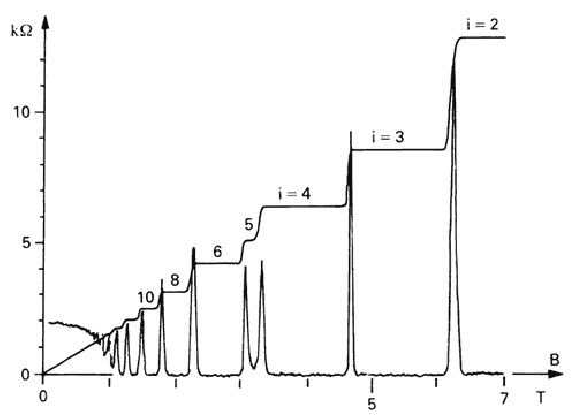
\includegraphics[width=\textwidth]{IntegerQHE.png}
		\caption{Integer quantum Hall effect (1980)}
	\end{subfigure}
	\hfill
	\begin{subfigure}[b]{0.3\textwidth}
		\centering
		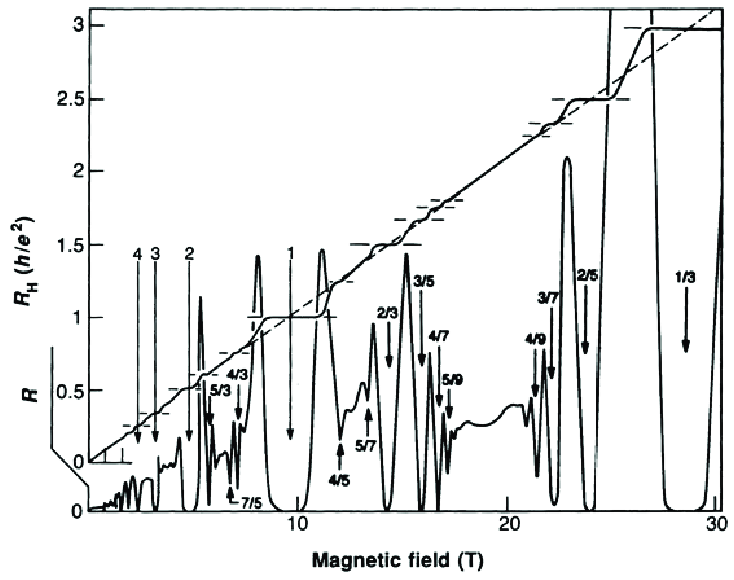
\includegraphics[width=\textwidth]{FractionalQHE.png}
		\caption{Fractional quantum Hall effect (1982)}
	\end{subfigure}
	\hfill
	\begin{subfigure}[b]{0.3\textwidth}
		\centering
		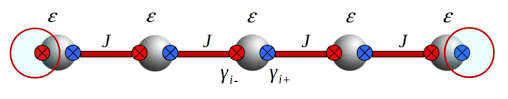
\includegraphics[width=\textwidth]{MajoranaEdgeModes.png}
		\caption{Majorana edge modes (first reported to be found in 2012 but data was not conclusive).}
	\end{subfigure}
	\caption{Three examples of topological order.}
	\label{fig:TopologicalOrderFigures}
\end{figure}
In 1980, Klaus von Klitzing drasticly changed the condensed matter physics landscape when he discovered a new phenomena called the integer quantum Hall effect. He applied an external magnetic field to a low temperature silicon based MOSFET and discovered that the Hall conductance induced by the magnetic field did not follow the classical linear dependence of this magnetic field. It in stead formed what we now call Hall plateaus (see figure \ref{fig:TopologicalOrderFigures}a). It was soon discovered that these plateaus where caused by new phases of matter that could not be distinguished by local order parameters breaking some symmetry and therefore did not follow Landaus paradigm. In later years many other such phases of matter emerged that did not follow the Landau paradigm. This included (and is not limited to) the fractional quantum Hall effect (see figure \ref{fig:TopologicalOrderFigures}b) and the majorana edge mode model\footnote{This is not found experimentally yet and is mainly theorized. There have been many experimental efforts to observe this effect but none of them have proven to be conclusive.} (see figure \ref{fig:TopologicalOrderFigures}c).\\\\
Theoretical descriptions of these new phases of matter looked very different from the old (Landau) phases of matter. As the name suggests the effect is quantum mechanical in nature. In fact it is related to a topological property of the gapped many body ground state. As such these phenomena area largely considered to be zero temperature phases of matter\footnote{With some caveats like the famous role of disorder that allows us to observe the quantum Hall plateaus in situations where there is no gap.}. For non interacting electrons in periodic potentials this topological property is the first Chern number of the Bloch bundle. For ground-states of more general interacting Hamiltonians the property that distinguishes the phases is much harder to distillate and in many ways (maybe this needs more information) still an open problem.\\\\
As these Hall plateaus where differentiated by some topological property of the many body ground-state they where called topological phases of matter. In the following years many such phases of matter where discovered all belonging to some topological property of some many body ground-state (sometimes multiple ground-states with some degeneracy). Just to name a few, there is invertible topological order (this is believed to be related to the integer quantum Hall effect), anyonic topological order (this is believed to be related to the fractional quantum Hall effect), symmetry protected topological order (this is related to the majorana edge modes), symmetry enriched topological order and many more.
\\\\
All of these topological phases of matter are described by a Hamiltonian that is gapped and a sum of local therms\footnote{In section \ref{sec:ToolsForQuantumManyBody} we will define these concepts in more detail.}\footnote{There are some caveats to this statement. For instance, one can still observe the quantum Hall effect in regimes where there is no gap.}. It turns out that this locality and this gap protects the topological orders mentioned at the end of the last section. To explain this more precisely we will define two equivalence classes: The first equivalence class is an equivalence on Hamiltonians:
\begin{definition}[Equivalence of Hamiltonians]\label{def:ConnectedHamiltonians}
	Two local Hamiltonians, with unique gapped ground-states, $H_0$ and $H_1$ are connected if there exists a path $t\mapsto H(t)$ such that
	\begin{itemize}
		\item $H(0)=H_0$ and $H(1)=H_1$.
		\item for each $t\in[0,1]$, $H(t)$ is a sum of local therms.
		\item each of the local therms of $H(t)$ is continuous in $t$.
	\end{itemize}
\end{definition}
The second equivalence class is an equivalence on states:
\begin{definition}[Equivalence of states]\label{def:ConnectedStates}
	Two states, $\ket{\psi_0}$ and $\ket{\psi_1}$ are connected if there exists a path $t\mapsto \ket{\psi(t)}$ with $\ket{\psi(0)}=\ket{\psi_0}$ and $\ket{\psi(1)}=\ket{\psi_1}$ such that there exists a one parameter family of local\footnote{By which we mean it is a sum of local therms.} Hermitian operators $K(s)$ such that
	\begin{align}
		\ket{\psi(t)}&=V(t)\ket{\psi(0)}&V(t)&=\mathcal{T}\exp(-i\int_{0}^{t}\d s K(s)).
	\end{align}
\end{definition}
In what follows we will call a unitary generated like this $V(t)$ a locally generated unitary (LGU).\\\\
Both these concepts are equivalent. More specifically:
\begin{itemize}
	\item If two uniquely gapped local Hamiltonians, $H_0$ and $H_1$, are equivalent through a path $H(t)$, the ground-states of $H(t)$ form a path satisfying what was in definition \ref{def:ConnectedStates}.
	\item If a state $\ket{\psi_0}$ is a unique gapped groundstate of some local Hamiltonian and is connected to $\ket{\psi_1}$ via a path $\ket{\psi(t)}$, there is a continuous path of parent Hamiltonians $H(t)$ for $\ket{\psi(t)}$ satisfying what was in definition \ref{def:ConnectedHamiltonians}.
\end{itemize}
We will provide the statements in more detail along with the main ideas needed for the proof in section \ref{sec:ToolsForQuantumManyBody}.\\\\
\begin{figure}
	\centering
	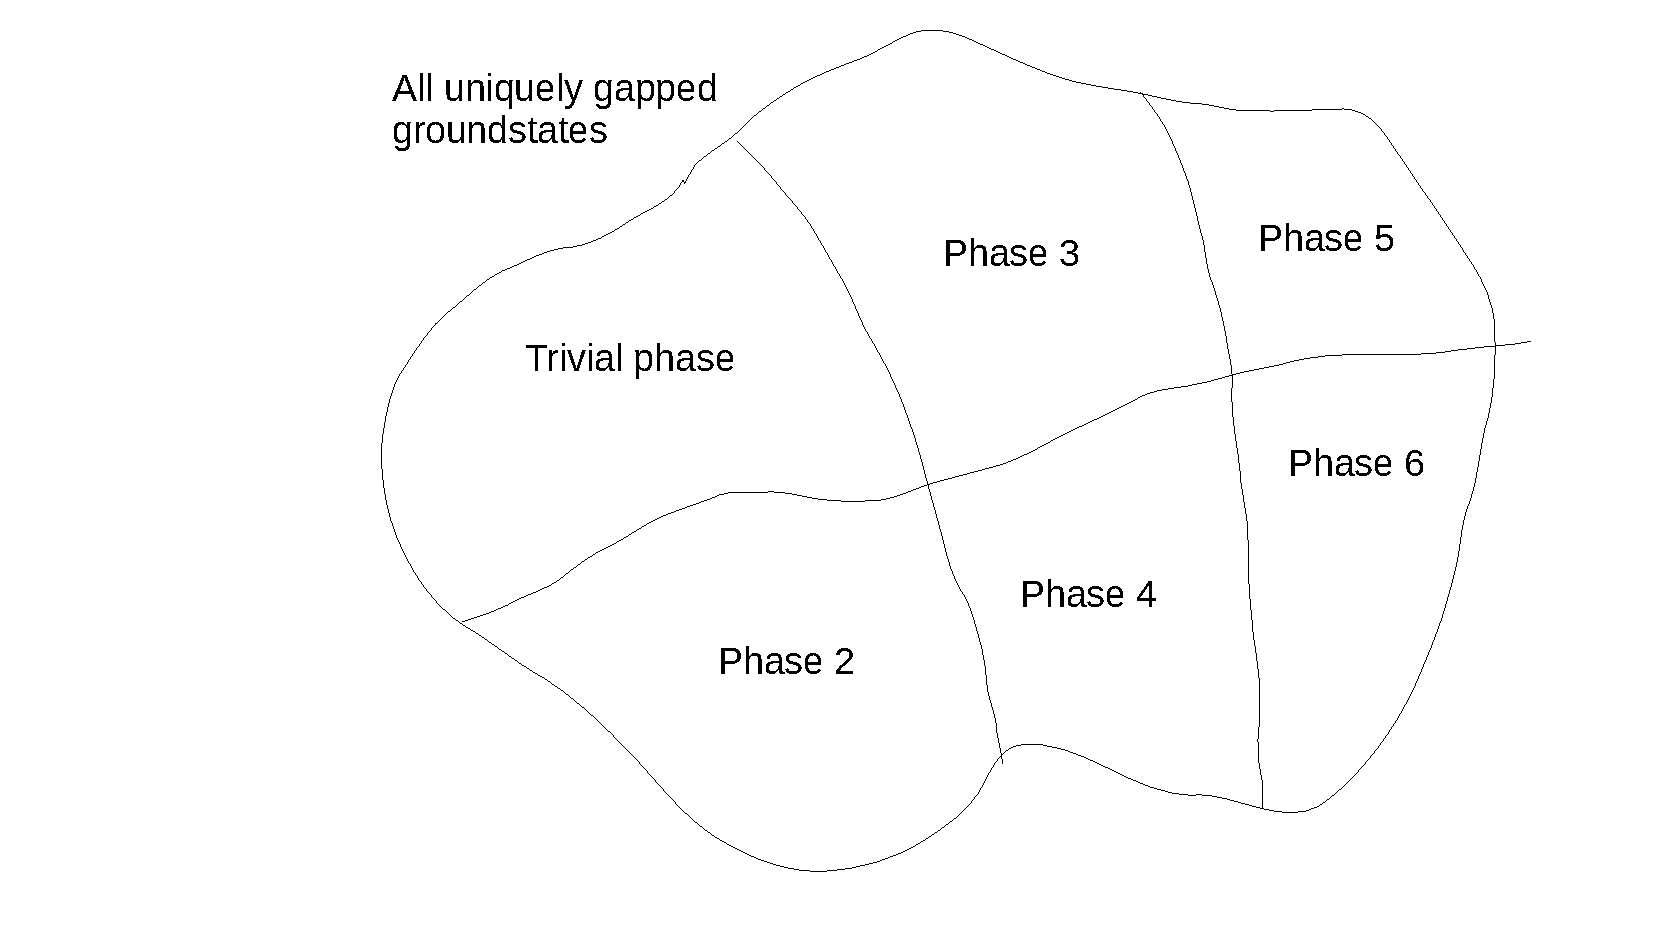
\includegraphics[width=0.8\textwidth]{GappedPhasesOfQuantumMatter.pdf}
	\caption{This is a graphical depiction of the quantum phases of matter. Any two states with different transverse Hall conductances have to be in different phases.}
	\label{fig:GappedPhasesOfQuantumMatter}
\end{figure}
These equivalence classes allow for a way to characterise these topological phases of matter. For example, if two of these states have different transverse Hall conductances they cannot be equivalent. We can try to generalise this. Suppose we take all states that can be written as the unique gapped ground-state of some local Hamiltonian and then tried to label all of the connected components with respect to the above equivalence class. These connected components are then called quantum phases of matter (see figure \ref{fig:GappedPhasesOfQuantumMatter}).
\section{Finite depth quantum circuits}\label{sec:finite-depth-quantum-circuits}
\begin{figure}
	\centering
	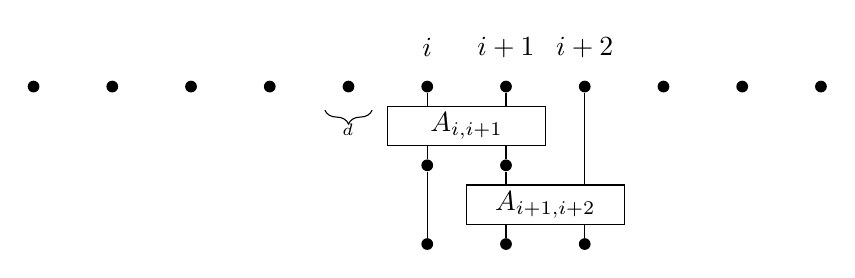
\begin{tikzpicture}
	\foreach \i in {1,...,11}
	{
		\node[circle,fill,inner sep=1.5pt] (\i) at (\i,0) {};
		
	}
	\node[] (i) at (6,0.5) {$i$};
	\node[] (i+1) at (7,0.5) {$i+1$};
	\node[] (i+2) at (8,0.5) {$i+2$};
	\draw [decorate,decoration={brace,amplitude=5pt},xshift=0cm,yshift=0pt] (5+0.3,-0.3) -- (5-0.3,-0.3) node [black,midway,yshift=-0.3cm] {\footnotesize $\CC^d$};
	
	
	\node[circle,fill,inner sep=1.5pt] (iDown) at (6,-1) {};
	\node[circle,fill,inner sep=1.5pt] (i+1Down) at (7,-1) {};
	\draw (6) -- (iDown);
	\draw (7) -- (i+1Down);
	\draw[fill=white] (5.5,-0.25) rectangle (7.5,-0.75);
	\node[] (A1) at (6.5,-0.5) {$A_{i,i+1}$};
	
	
	\node[circle,fill,inner sep=1.5pt] (iFarDown) at (6,-2) {};
	\node[circle,fill,inner sep=1.5pt] (i+1FarDown) at (7,-2) {};
	\node[circle,fill,inner sep=1.5pt] (i+2FarDown) at (8,-2) {};
	\draw (iDown)--(iFarDown);
	\draw (i+1Down)--(i+1FarDown);
	\draw (8)--(i+2FarDown);
	\draw[fill=white] (6.5,-1.25) rectangle (8.5,-1.75);
	\node[] (A1) at (7.5,-1.5) {$A_{i+1,i+2}$};
	
	
\end{tikzpicture}
	\caption{This figure shows a one dimensional lattice. It then also shows the algebraic structure of local operators. If one multiplies a an operator with support on $\{i,i+1\}$ with an operator having support on $\{i+1,i+1\}$, one obtains an operator having support on $\{i,i+1,i+2\}$.}
	\label{fig:Lattice}
\end{figure}
\begin{figure}
	\centering
	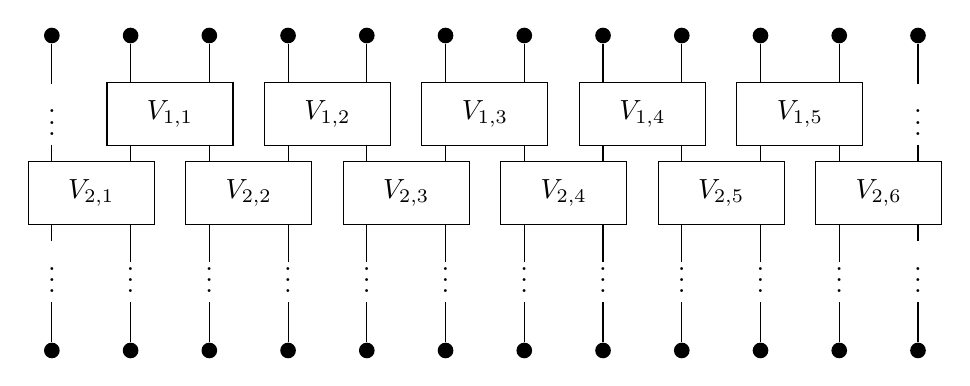
\begin{tikzpicture}
	\foreach \x in {0,...,11}{
		\node (\x) [circle,fill,inner sep=2pt] at (\x,0) {};
		\node (3\x) [circle,fill,inner sep=2pt] at (\x,-2) {};
		\node (4\x) [] at (\x,-3) {$\vdots$};
		\node (5\x) [circle,fill,inner sep=2pt] at (\x,-4) {};
	}
	
	\foreach \x in {1,...,10}{
		\node (2\x) [] at (\x,-3) {};
	}
	\node (20) at (0,-1) {$\vdots$};
	\node (211) at (11,-1) {$\vdots$};
	
	\foreach \x in {0,...,11}{
		\draw (\x) -- (2\x);
		\draw (2\x) -- (3\x);
		\draw (3\x) -- (4\x);
		\draw (4\x) -- (5\x);
	}
	
	\foreach \x in {1,...,5}
	\draw [fill=white] (2*\x-0.3-1,-0.6) rectangle (2*\x+0.3,-1.4);
	\foreach \x in {0,...,5}
	\draw [fill=white] (2*\x-0.3,-1.6) rectangle (2*\x+0.3+1,-2.4);
	
	\foreach \x in {1,...,5}
	\node [] at (2*\x-0.5,-1) {$V_{1,\x}$};
	\foreach \x in {0,...,5}
	\node [] at (2*\x+0.5,-2) {$V_{2,\pgfmathtruncatemacro\result{\x+1}\result}$};
	
	
\end{tikzpicture}
	\caption{Example of a finite depth quantum circuit with two layers being displayed.}
	\label{fig:FiniteDepthQuantumCirquit}
\end{figure}
In this section we will define a particularly simple set of examples of these LGU's called finite depth quantum circuits (FDQC). To examine what they are, envision one has a lattice $\Lambda$. In figure \ref{fig:Lattice} we give a graphical depiction of a one dimensional lattice\footnote{All of the definitions in this section however can be generalised to other lattices.}. A lattice is a collection of sites. To each site we attach a Hilbert space, say $\CC^d$ (for some small integer $d$). The full Hilbert space is then $\HH=\bigotimes_{i\in\Lambda}\CC^d$\footnote{For infinite lattices like $\Lambda=\ZZ$ or $\Lambda=\ZZ^2$, this does Hilbert space cannot be defined. More on this in section \ref{sec:ToolsForQuantumManyBody}.}. One then defines a local operator as an operator that acts on the tensor product of a few sites and acts trivially on the other sites (these sites are then called the support of the operator). These local operators form an algebra as multiplying two local operators gives a new local operator (an example of this is given in figure \ref{fig:Lattice}).\\\\
We now create a unitary on this full Hilbert space of the following form (see figure \ref{fig:FiniteDepthQuantumCirquit} for a graphical depiction). We first create an even layer which is an operator of the form $V_1=\bigotimes_{i}V_{1,i}$ where $V_{1,i}$ has support on sites $2i$ and $2i+1$. Next we create an odd layer which is of the same form only $V_{2,i}$ has support on sites $2i-1$ and $2i$. A unitary that is a product of odd layers and even layers is called a finite depth quantum circuit (FDQC). The amount of layers used is then called the depth. So a circuit of depth $D$ is a unitary of the form $V_D\cdots V_1$ where the $V_i$ alternate between even and odd layers.\\\\
\begin{figure}
	\centering
	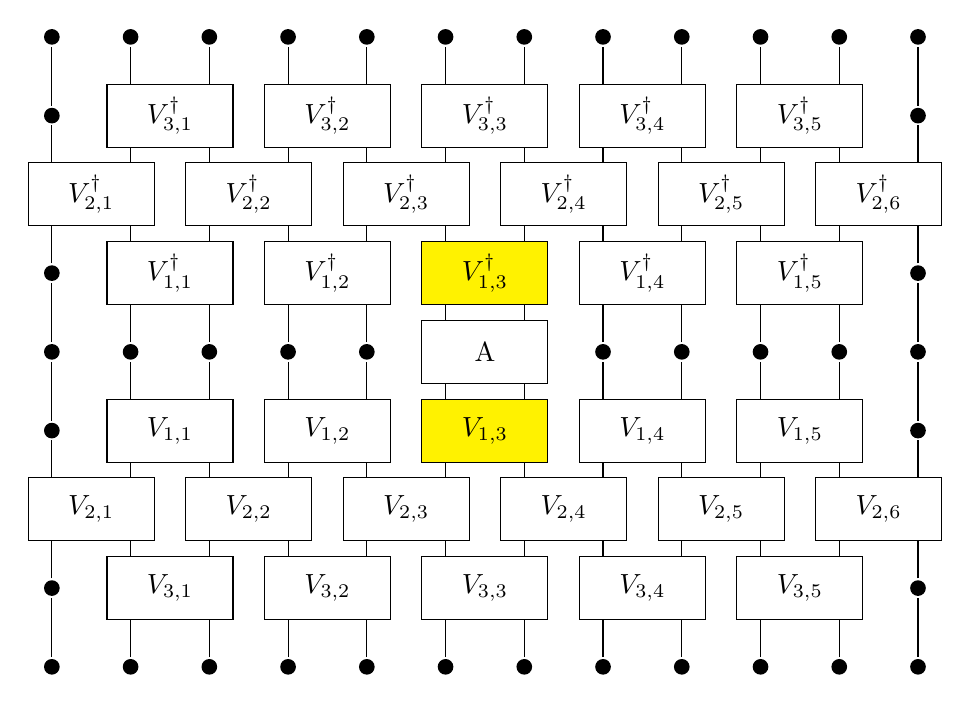
\begin{tikzpicture}
	\foreach \x in {0,...,11}{
		\foreach \y in {-4,...,4}{
			\ifthenelse{\y=-4 \OR \y=4}{\node (\y \x) [circle,fill,inner sep=2pt] at (\x,\y) {};}
			{\node (\y \x) [] at (\x,\y) {};}
		}
	}
	
	
	\foreach \x in {0,...,11}{
		\foreach \y in {-4,...,3}{
			\draw (\y \x) -- (\the\numexpr \y + 1\relax \x);
		}
	}

	\draw[fill=white] (4.7,0.4) rectangle (6.3,-0.4);
	\node at (5.5,0) {A};
	
	\foreach \x in {1,...,5}{
	\if\x3{
		\draw [fill=yellow] (2*\x-0.3-1,-0.6) rectangle (2*\x+0.3,-1.4);
		\draw [fill=yellow] (2*\x-0.3-1,0.6) rectangle (2*\x+0.3,1.4);
	}
	\else{
		\draw [fill=white] (2*\x-0.3-1,-0.6) rectangle (2*\x+0.3,-1.4);
		\draw [fill=white] (2*\x-0.3-1,0.6) rectangle (2*\x+0.3,1.4);
	}\fi};
	
	\foreach \x in {0,...,5}{
		\ifthenelse{\x=2 \OR \x=3}{\draw [fill=yellow] (2*\x-0.3,-1.6) rectangle (2*\x+0.3+1,-2.4);}{\draw [fill=white] (2*\x-0.3,-1.6) rectangle (2*\x+0.3+1,-2.4);}
		\ifthenelse{\x=2 \OR \x=3}{\draw [fill=yellow] (2*\x-0.3,1.6) rectangle (2*\x+0.3+1,2.4);}{\draw [fill=white] (2*\x-0.3,1.6) rectangle (2*\x+0.3+1,2.4);}
	};
	\foreach \x in {1,...,5}{
		\ifthenelse{\x=2 \OR \x=3 \OR \x=4}{\draw [fill=yellow] (2*\x-0.3-1,-2.6) rectangle (2*\x+0.3,-3.4);}{\draw [fill=white] (2*\x-0.3-1,-2.6) rectangle (2*\x+0.3,-3.4);}
		\ifthenelse{\x=2 \OR \x=3 \OR \x=4}{\draw [fill=yellow] (2*\x-0.3-1,2.6) rectangle (2*\x+0.3,3.4);}{\draw [fill=white] (2*\x-0.3-1,2.6) rectangle (2*\x+0.3,3.4);}
	}
	
	\foreach \x in {1,...,5}{
		\node [] at (2*\x-0.5,-1) {$V_{1,\x}$};
		\node [] at (2*\x-0.5,-3) {$V_{3,\x}$};
		\node [] at (2*\x-0.5,1) {$V_{1,\x}^\dagger$};
		\node [] at (2*\x-0.5,3) {$V_{3,\x}^\dagger$};
	}
	\foreach \x in {0,...,5}{
		\node [] at (2*\x+0.5,-2) {$V_{2,\the\numexpr \x + 1\relax}$};
		\node [] at (2*\x+0.5,2) {$V_{2,\the\numexpr \x + 1\relax}^\dagger$};
	}
	
	
\end{tikzpicture}

	\caption{This figure displays the operator $\Ad{V}(A)$ where $V$ is a finite depth quantum cirquit and $A$ is an operator with small support. The only unitaries in the FDQC that contribute in $\Ad{V}(A)$ are indicated in yellow. The other ones will cancel with the coresponding unitaries in $V^\dagger$. In general this implies that the diameter of the support of $\Ad{V}(A)$ is bounded by $\text{diam}(A)+2D$.}
	\label{fig:FiniteDepthQuantumCirquitLightcone}
\end{figure}
In this setting, one should think of the depth $D$ as being a lot smaller than the total amount of sites $L$. In this case a quantum circuit has two very important properties that we want to use. The first one is that a FDQC is indeed an LGU. This can be easily seen from the fact that for any of the local unitaries $V_{i,j}\in\UU(\CC^d\otimes\CC^d)$, we can find a Hermitian operator $K_{i,j}\in\textrm{Herm}(\CC^d\otimes\CC^d)$ such that
\begin{equation}
	V_{i,j}=\exp(-i K_{i,j}).
\end{equation}
If we now define the sum of local therms operator
\begin{equation}
	K(s)\defeq \left\{\begin{matrix}
		\sum_{j}(K_{1,j})_{2j,2j+1}&\text{if }0<s<1/D\\
		\sum_{j}(K_{2,j})_{2j-1,2j}&\text{if }1/D<s<2/D\\
		\vdots&\vdots
	\end{matrix}\right.
\end{equation}
(here $D$ was the depth of the FDQC) then we indeed obtain that
\begin{equation}
	V=\mathcal{T}\exp(-iD\int_0^1 \d s K(s)).
\end{equation}
This means in particular that any two states that are connected through a FDQC are also connected as in definition \ref{def:ConnectedStates}. Moreover the depth is linearly proportional to the norm of the required Hamiltonian.\\\\
The second one is that a FDQC preserves the locality of operators. More specifically we will show that the diameter of the support of $\Ad{V}(A)$ (with $V$ a finite depth quantum cirquit) grows only linearly with the depth of $V$. To see this take an operator $A$ with support contained in some diameter $\text{diam}(A)$. As is shown in figure \ref{fig:FiniteDepthQuantumCirquitLightcone}, if one now works out $\Ad{V}(A)$ one observes that this operator only depends on the unitaries in a particular lightcone around the support of $A$. This implies that the diameter of the support of $\Ad{V}(A)$ is bounded by $\text{diam}(A)+2D$. This means that a FDQC preserves the locality of operators. There is a generalisation of this signal locality (as it is sometimes called) to any LGU. This generalisation is called the Lieb Robinson bound and is described in section \ref{sec:ToolsForQuantumManyBody}.
\section{Enriching the trivial phase with symmetry}\label{sec:enriching-the-trivial-phase-with-symmetry}
\begin{figure}
	\centering
	\scalebox{0.9}{
		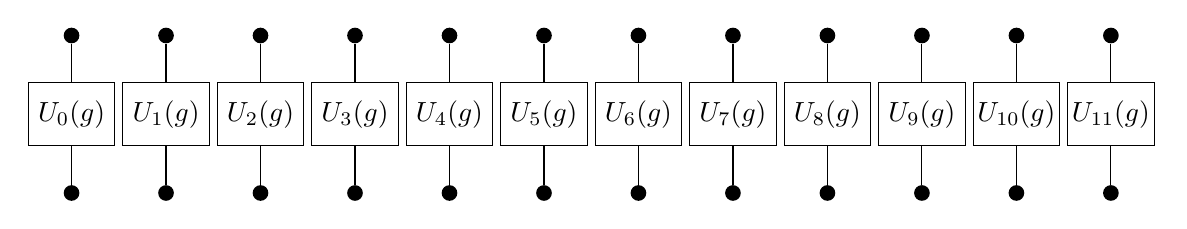
\begin{tikzpicture}
	\foreach \x in {0,...,11}{
		\node (\x) [circle,fill,inner sep=2pt] at (\x*1.2,0) {};
		\node (2\x) [] at (\x*1.2,-1) {};
		\node (3\x) [circle,fill,inner sep=2pt] at (\x*1.2,-2) {};
	}
	
	\foreach \x in {0,...,11}{
		\draw (\x) -- (2\x);
		\draw (2\x) -- (3\x);
	}
	
	\foreach \x in {0,...,11}
	\draw [fill=white] (\x*1.2-0.55,-0.6) rectangle (\x*1.2+0.55,-1.40);
	
	\foreach \x in {0,...,11}{
		\node (other \x) [] at (\x*1.2,-1) {$U_{\x}(g)$};
	}
\end{tikzpicture}
	}
	\caption{This figure shows the group action as a finite depth quantum cirquit.}
	\label{fig:GroupActionQuantumCirquit}
\end{figure}
\begin{figure}
	\centering
	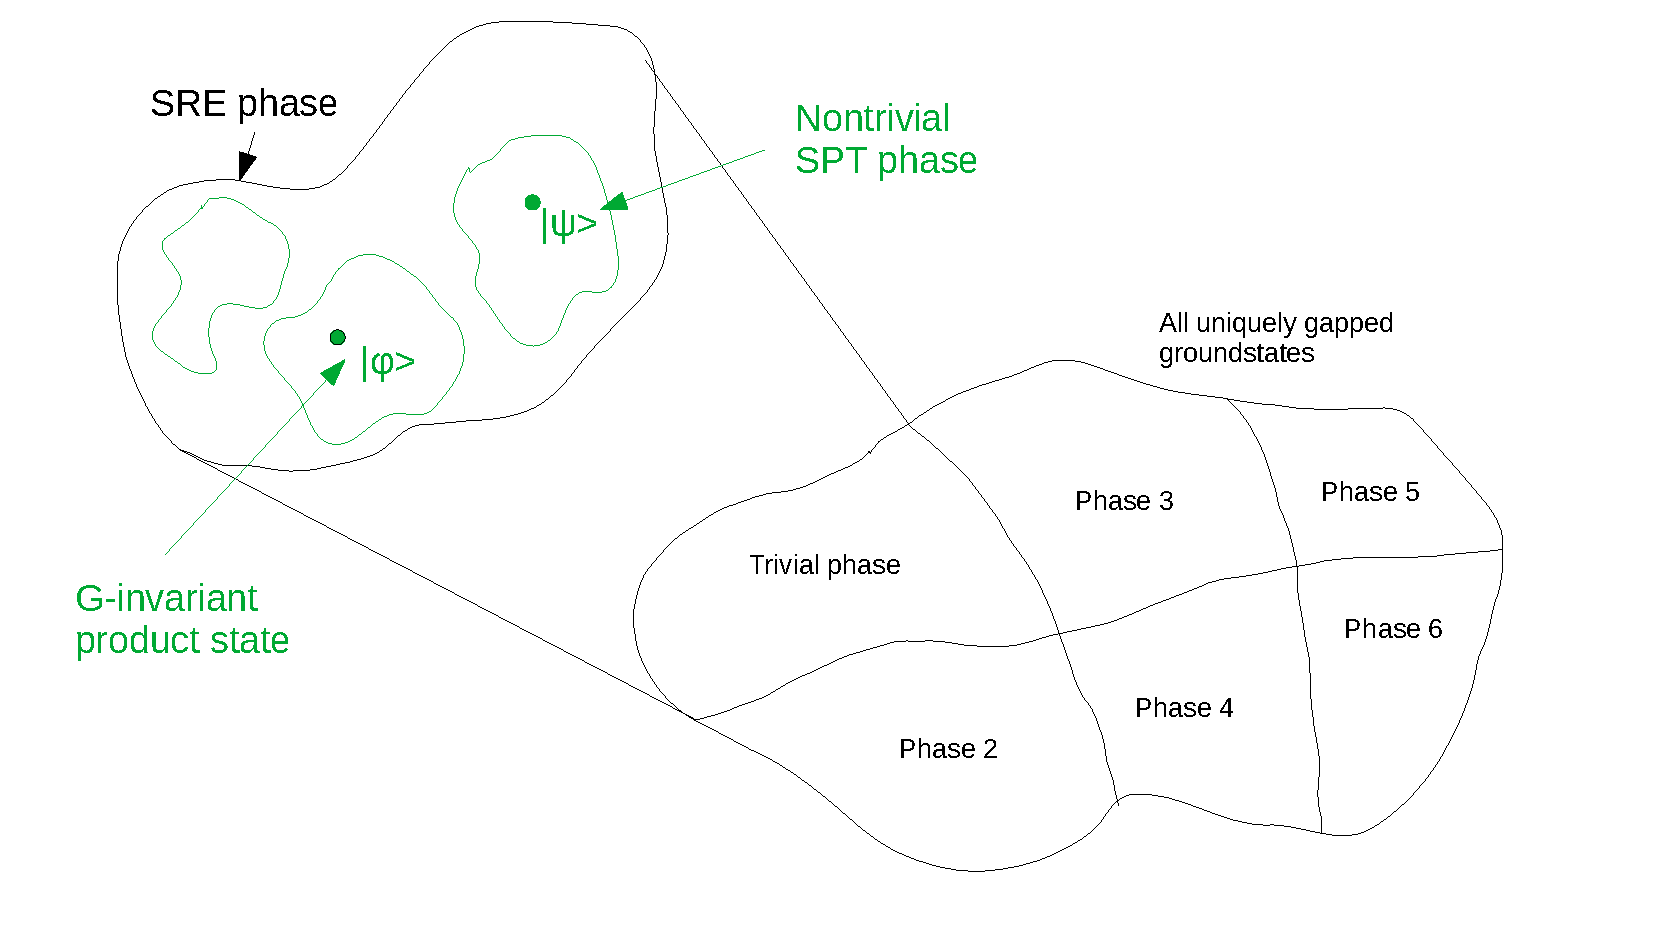
\includegraphics[width=0.8\textwidth]{SPT_Phases.pdf}
	\caption{This figure shows all states connected to some trivial product state $\ket{\phi}$. The highlighted black area displays all states connected to $\ket{\phi}$ via a generic LGU while the green areas show the $G$-invariant states that are connected to each other via a $G$-invariant LGU.}
	\label{fig:ConnectedComponents}
\end{figure}
FDQCs give a first way to compare topological phases of matter. If two many body groundstates can be mapped into one another via a FDQC, they are in the same quantum phase of matter. It now makes sense to look at what the trivial quantum phase of matter looks like (in the Landau picture the trivial phase was the symmetry preserving phase). To this end we first define the most trivial state we can think of which is called the product state. It is the only state that has no entanglement between any of its sites. On the Hilbert space above one could define a product state by fixing a vector $\ket{v_i}\in\CC^d$ for each lattice site $i$ and defining $\ket{\phi_0}=\bigotimes_{i\in\Lambda}\ket{v_i}$. We now call a state $\ket{\psi}\in\HH$, short range entangled (SRE) if there exists an LGU, $U$ such that $\ket{\psi}=U\ket{\phi_0}$.\\\\
These SRE states then form by construction the topologically trivial quantum phase of matter. They can in a local and smooth way be deformed to the most trivial state of all. The kind of topological order that we will discus in this thesis is precisely the topological order that emerges when one applies an additional symmetry to this trivial phase. To this end, take a group $G$\footnote{Later on we will only talk about finite groups but for now the reader can think of any compact Lie Group.}. Now for each site $i$, take a unitary representation on the on site Hilbert space $U_i\in\hom(G,U(\CC^d))$. Use this to define a representation on the full Hilbert $U\in\hom(G,U(\HH))$ such that $U(g)=\bigotimes_{i\in\Lambda}U_i(g)$. If we graphically depict this in the same way as we did for the finite depth quantum cirquits it looks like in figure \ref{fig:GroupActionQuantumCirquit}.\\\\
We now call an SRE state $\ket{\psi}$, $G$-invariant if $U(g)\ket{\psi}=\ket{\psi}$ for all $g\in G$. We will put a similar but slightly stronger condition on product states and say that a product state $\ket{\phi_0}$ is $G$-trivial if $U_i(g)\ket{\phi_0}=\ket{\phi_0}$ for all $i\in\Lambda$ and all $g\in G$. Finally we call a FDQC, $G$-invariant if each of the unitaries $U_{ij}$ in the FDQC commutes with the group action $U(g)$. Equivalently a FDQC is $G$-invariant if each of its layers commutes with the group action.\\\\
We can now define SPT phases through the following procedure (see figure \ref{fig:ConnectedComponents}). First, pick a $G$-trivial product state $\ket{\phi_0}$. Take all states connected to $\ket{\phi_0}$ via some finite depth quantum cirquit. Now out of those states pick only the $G$-invariant ones and group them together if they can be connected via a $G$-invariant FDQC. The groups obtained are now called the SPT phases.
\section{Zero dimensional SPTs}\label{sec:zero-dimensional-spts}The first example that we will give is when the lattice is trivial $\Lambda=\{1\}$. In this case the total Hilbert space is the same as the on site Hilbert space and the group action $U\in\hom(G,U(\CC^d))$ is just a finite dimensional representation. A state $\ket{\psi}\in\CC^d$ is then $G$-invariant if there exists an $\alpha:G\rightarrow U(1)$ such that
\begin{equation}
	U(g)\ket{\psi}=\alpha(g)\ket{\psi}.
\end{equation}
However, since
\begin{equation}
	U(g)U(h)\ket{\psi}=U(gh)\ket{\psi}
\end{equation}
we need that $\alpha(g)\alpha(h)=\alpha(gh)$ and therefore $\alpha\in\hom(G,U(1))$. The trivial state is then the state such that $\alpha=1$. We therefore say that the zero dimensional SPTs are classified by the $U(1)$-representations $\hom(G,U(1))$. We will see in subsection \ref{sec:example-1-h1gtt} that this group is the same as something called the first group cohomology group.
\section{An example in 1d: The Haldane phase}
The next example is a slightly less trivial one. We will now take the one dimensional lattice $\Lambda=\ZZ$.\footnote{As discussed before, this means the full Hilbert space is not a well defined object. We will for now however chose to ignore this and revisit it in section \ref{sec:ToolsForQuantumManyBody}.} In this example we will take as group $\ZZ_2\times\ZZ_2$\footnote{We can extend this group in a straightforward way to $SO(3)$ using the double covering, $f:SU(2)\rightarrow SO(3)$.}. We write the four group elements of $\ZZ_2\times\ZZ_2$ as
\begin{align}
	&(1,1)&&(-1,1)&&(1,-1)&&(-1,-1).
\end{align}
The group multiplication is then given by pointwise multiplication of these numbers.
\subsection{The on site group action}
As on site Hilbert space we take $\CC^4\cong \CC^2\otimes\CC^2$. As on site group action we take the unitary representation $u:\ZZ_2\times\ZZ_2\rightarrow U(\CC^2\otimes\CC^2)$ defined through
\begin{align}\label{eq:OnSiteActionOfFakeAKLT_Model}
	u(1,1)&=\id_{\CC^4}&u(-1,1)&=-\sigma_x\otimes\sigma_x&u(1,-1)&=-\sigma_y\otimes\sigma_y&u(-1,-1)&=-\sigma_z\otimes\sigma_z.
\end{align}
We then take a copy of this unitary for each site and this gives our group action $U(g)=\bigotimes_{i=1}^{L}u(g)$. Finally we will need to define a basis for $\CC^4$ that we will use to define our state in. We will take the singlet and triplet basis:
\begin{align}
	&&\ket{s}&=\frac{1}{\sqrt{2}}(\ket{\uparrow\downarrow}-\ket{\downarrow\uparrow})&&\\
	\ket{0}&=\frac{1}{\sqrt{2}}(\ket{\uparrow\downarrow}+\ket{\downarrow\uparrow})&\ket{-1}&=\ket{\downarrow\downarrow}&\ket{1}&=\ket{\uparrow\uparrow}.
\end{align}
The singlet is now invariant under the group action ($u(g)\ket{s}=\ket{s}$ for all $g\in G$) while the group action acts irreducibly on the three triplet vectors.
\subsection{Intermezzo: Linear and projective representations}
I can rewrite the unitaries in equation \eqref{eq:OnSiteActionOfFakeAKLT_Model} as
\begin{align}\label{eq:OnSiteActionOfFakeAKLT_Model_Rewritten}
	u(1,1)&=\id_{\CC^2}\otimes\id_{\CC^2}&u(-1,1)&=(i\sigma_x)\otimes(i\sigma_x)&u(1,-1)&=(i\sigma_y)\otimes(i\sigma_y)&u(-1,-1)&=(i\sigma_z)\otimes(i\sigma_z).
\end{align}
One could therefore wonder whether
\begin{align}\label{eq:OnSiteActionOfFakeAKLT_Model_OnC2}
	r(1,1)&=\id_{\CC^2}&r(-1,1)&=i\sigma_x&r(1,-1)&=i\sigma_y&r(-1,-1)&=i\sigma_z
\end{align}
is a representation. It turns out this is not the case. This can easily be seen by the fact that $r(-1,1)$ and $r(1,-1)$ don't commute. $r$ does however commute up to a phase. More specifically, define $[\cdot]_\sim$ as the equivalence class that says that two operators are equivalent if they differ only up to a phase. Then $\tilde{r}$, defined through
\begin{align}\label{eq:OnSiteActionOfFakeAKLT_Model_OnC2_ProjectiveRep}
	\tilde r(1,1)&=[\id_{\CC^2}]_\sim&\tilde r(-1,1)&=[\sigma_x]_\sim\\
	\tilde r(1,-1)&=[\sigma_y]_\sim&\tilde r(-1,-1)&=[\sigma_z]_\sim
\end{align}
is a representation ($\tilde{r}\in\hom(G,\PP\UU(\CC^2))$). We call such an $\tilde{r}$ a projective representation and we call $r$ then the lift of a projective representation.
\subsection{The trivial product state and the entangled pair state}
\begin{figure}
	\centering
	\begin{subfigure}{\textwidth}
		\centering
		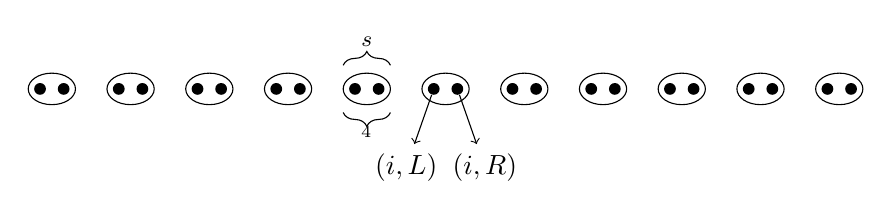
\begin{tikzpicture}
	\foreach \i in {1,...,11}
	{
		\draw[black] (\i,0) ellipse (0.3 and 0.2);
		\node (\i L) [circle,fill,inner sep=1.5pt] at (\i-0.15,0) {};
		\node (\i R) [circle,fill,inner sep=1.5pt] at (\i+0.15,0) {};
		
	}
	\draw [decorate,decoration={brace,amplitude=5pt},xshift=0cm,yshift=0pt] (5-0.3,0.3) -- (5+0.3,0.3) node [black,midway,yshift=0.3cm] {\footnotesize $\ket{s}$};
	\draw [decorate,decoration={brace,amplitude=5pt},xshift=0cm,yshift=0pt] (5+0.3,-0.3) -- (5-0.3,-0.3) node [black,midway,yshift=-0.3cm] {\footnotesize $\CC^4$};
	\node (iL) [] at (5.5,-1) {$(i,L)$};
	\draw[black,->] (6L) -- (iL);
	\node (iR) [] at (6.5,-1) {$(i,R)$};
	\draw[black,->] (6R) -- (iR);
	
\end{tikzpicture}
		\caption{The trivial product state.}
		\label{fig:TrivialProductState}
	\end{subfigure}
	\begin{subfigure}{\textwidth}
		\centering
		\begin{tikzpicture}
	\foreach \i in {1,...,10}
	{
		\draw[black] (\i+0.5,0) ellipse (0.48 and 0.2);
		\filldraw [black] (\i-0.15,0) circle (2pt);
		\filldraw [black] (\i+0.15,0) circle (2pt);
	}
	\filldraw [black] (11-0.15,0) circle (2pt);
	\filldraw [black] (11+0.15,0) circle (2pt);
	\draw [decorate,decoration={brace,amplitude=5pt},xshift=0cm,yshift=0pt] (5,0.3) -- (5+1,0.3) node [black,midway,yshift=0.3cm] {\footnotesize $\ket{s}$};
	\draw [decorate,decoration={brace,amplitude=5pt},xshift=0cm,yshift=0pt] (5+0.3,-0.3) -- (5-0.3,-0.3) node [black,midway,yshift=-0.3cm] {\footnotesize $\CC^4$};
	\begin{scope}
		\clip(0.5,0.2)rectangle(1,-0.2);
		\draw[black] (0.5,0) ellipse (0.48 and 0.2);
	\end{scope}
	\begin{scope}
		\clip(11,0.2)rectangle(11.5,-0.2);
		\draw[black] (11.5,0) ellipse (0.48 and 0.2);
	\end{scope}
	\node (iL) [] at (5.5,-1) {$(i,L)$};
	\draw[black,->] (6L) -- (iL);
	\node (iR) [] at (6.5,-1) {$(i,R)$};
	\draw[black,->] (6R) -- (iR);
\end{tikzpicture}
		\caption{The entangled pair state.}
		\label{fig:FakeAKLT_State}
	\end{subfigure}
	\caption{These are two $\ZZ_2\times\ZZ_2$ invariant states. The first one is a trivial state the other one is an SRE state. Each dot represents the Hilbert space $\CC^2$, each circle indicates that out of $\CC^2\otimes\CC^2$, the singlet state is chosen. The dots that are near each other form a site.}
	\label{fig:TheTwoHaldanePhases}
\end{figure}
Now we define the trivial product state. As $\ket{s}$ was the only invariant vector in $\CC^4$ the trivial product state is simply $\ket{\phi}=\bigotimes_{i\in\Lambda}\ket{s}_{i_L,i_R}$. Figure \ref{fig:TrivialProductState} gives a graphical representation of this state. In a similar fashion we can also construct a nontrivial state. We simply take $\ket{\psi}=\bigotimes_{i\in\Lambda}\ket{s}_{i_R,(i+1)_L}$\footnote{For open boundary conditions, we did not specify what we do with $1_L$ and $L_R$. In fact this state can only be made $G$ invariant if one places it in periodic boundary conditions or if one defines it on the infinite lattice (which is what we will do later on in the thesis).}. We call this state the entangled pair state\footnote{This is related to the AKLT statem named after this paper: \cite{PhysRevLett.59.799}. It differs from the real AKLT state in that we only construct the entangled pairs here, we don't project the sites to the triplets.} state. This state is also a product of $G$-invariant states and is therefore by construction $G$-invariant as well.\\\\
I constructed two $G$-invariant states. One of them is a trivial product state. Now I would like to argue that the other state is a state with nontrivial SPT order. To do this I must do two things.
\begin{enumerate}
	\item I have to show that they can be connected via a finite depth quantum cirquit.
	\item I have to show that they cannot be connected via a $G$-invariant finite depth quantum cirquit.
\end{enumerate}
\begin{figure}
	\centering
	\begin{tikzpicture}
		\foreach \i in {1,...,11}
	{
		\draw[black] (\i,0) ellipse (0.3 and 0.2);
		\foreach \j in {0,...,3}{
			\node (Left\i\j) [circle,fill,inner sep=1.6pt] at (\i-0.15,-2*\j) {};
			\node (Right\i\j) [circle,fill,inner sep=1.6pt] at (\i+0.15,-2*\j) {};
		}
	}
	\newcommand\y{6}
	
	\foreach \i in {1,...,10}
	{
		\draw[black] (\i+0.5,-\y) ellipse (0.48 and 0.2);
	}
	\begin{scope}
		\clip(0.5,-\y+0.2)rectangle(1,-\y-0.2);
		\draw[black] (0.5,-\y) ellipse (0.48 and 0.2);
	\end{scope}
	\begin{scope}
		\clip(11,-\y+0.2)rectangle(11.5,-\y-0.2);
		\draw[black] (11.5,-\y) ellipse (0.48 and 0.2);
	\end{scope}

	\foreach \i in {1,...,11}
	{
		\draw (Left\i0) -- (Left\i1);
		\draw (Right\i0) -- (Right\i1);
		\ifthenelse{\isodd{\i}}{
			\draw (Right\i1) -- (Right\i2);
			\draw (Left\i2) -- (Left\i3);
		}{
			\draw (Left\i1) -- (Left\i2);
			\draw (Right\i2) -- (Right\i3);
		}
	}
	\foreach \i in {1,...,11}{
		\draw[fill=white] (\i-0.4,-0.4) rectangle (\i+0.4,-1.4);
		\node[] (\i) at (\i,-1) {$U$};
		\ifthenelse{\isodd{\i}}{
			\draw[fill=white] (\i,-2.6) rectangle (\i+1,-3.4);
			\node[] (SecondUnitary\i) at (\i+0.5,-3) {$U^\dagger$};
			\draw[fill=white] (\i-1,-4.6) rectangle (\i,-5.4);
			\node[] (ThirdUnitary\i) at (\i-0.5,-5) {$U^\dagger$};
			\draw[black] (\i+0.5,-4) ellipse (0.48 and 0.2);
		}{}
	}
\end{tikzpicture}
	\caption{This figure displays a finite depth quantum cirquit of depth 3 mapping the trivial product state to the entangled pair state. As before the curves indicate singlet states and the dots without curves around them indicate $\ket{\uparrow}$ states. The $U$ here is therefore a unitary on $\CC^4$ that maps the $\ket{s}$ state to the $\ket{1}=\ket{\uparrow\uparrow}$ state.}
	\label{fig:FakeAKLT_IsSRE}
\end{figure}
To show the first point, first let $U$ be a unitary on $\CC^4$ that maps $\ket{s}$ to $\ket{1}=\ket{\uparrow\uparrow}$. I now create a finite depth quantum cirquit $V$ consisting of three layers. Look at figure \ref{fig:FakeAKLT_IsSRE} for a schematic picture of the layers of $V$. The first layer is both odd and even, $V_1=\bigotimes_{i\in\Lambda}U_{i_L,i_R}$ (it rotates the sites themselves). The second layer is odd, $V_2=\bigotimes_{i\in\Lambda}U_{(2i-1)_R,2i_L}^\dagger$. The third layer is even, $V_3=\bigotimes_{i\in\Lambda}U_{2i_R,(2i+1)_L}^\dagger$. This concludes our FDQC.
\subsection{The product state transforms linearly while the entangled pair state transforms projectively}
\begin{figure}
	\centering
	\begin{subfigure}{\textwidth}
		\centering
		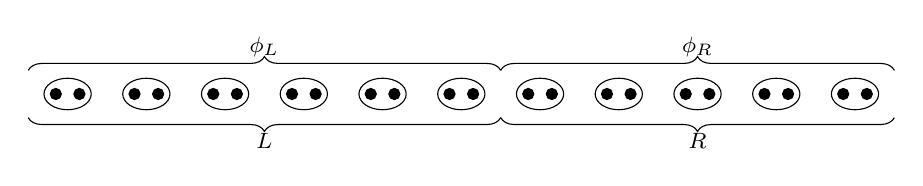
\begin{tikzpicture}
	\foreach \i in {1,...,11}
	{
		\draw[black] (\i,0) ellipse (0.3 and 0.2);
		\filldraw [black] (\i-0.15,0) circle (2pt);
		\filldraw [black] (\i+0.15,0) circle (2pt);
		
	}
	\draw [decorate,decoration={brace,amplitude=5pt},xshift=0cm,yshift=0pt] (6.5,0.3) -- (11.5,0.3) node [black,midway,yshift=0.3cm] {\footnotesize $\ket{\phi_{R}}$};
	\draw [decorate,decoration={brace,amplitude=5pt},xshift=0cm,yshift=0pt] (0.5,0.3) -- (6.5,0.3) node [black,midway,yshift=0.3cm] {\footnotesize $\ket{\phi_{L}}$};
	\draw [decorate,decoration={brace,amplitude=5pt},xshift=0cm,yshift=0pt] (6.5,-0.3) -- (0.5,-0.3)  node [black,midway,yshift=-0.3cm] {\footnotesize $L$};
	\draw [decorate,decoration={brace,amplitude=5pt},xshift=0cm,yshift=0pt] (11.5,-0.3) -- (6.5,-0.3)  node [black,midway,yshift=-0.3cm] {\footnotesize $R$};
\end{tikzpicture}
		\caption{The trivial product state.}
		\label{fig:TrivialProductStateTwoParts}
	\end{subfigure}
	\begin{subfigure}{\textwidth}
		\centering
		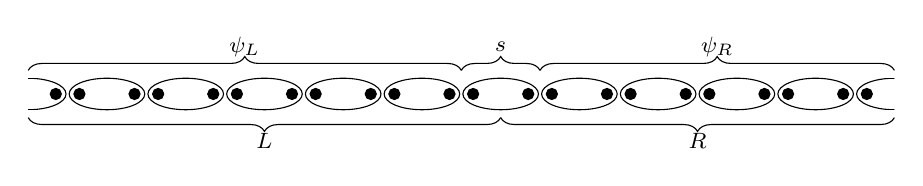
\begin{tikzpicture}
	\foreach \i in {1,...,10}
	{
		\draw[black] (\i+0.5,0) ellipse (0.48 and 0.2);
		\filldraw [black] (\i-0.15,0) circle (2pt);
		\filldraw [black] (\i+0.15,0) circle (2pt);
		
	}
	\filldraw [black] (11-0.15,0) circle (2pt);
	\filldraw [black] (11+0.15,0) circle (2pt);
	\begin{scope}
		\clip(0.5,0.2)rectangle(1,-0.2);
		\draw[black] (0.5,0) ellipse (0.48 and 0.2);
	\end{scope}
	\begin{scope}
		\clip(11,0.2)rectangle(11.5,-0.2);
		\draw[black] (11.5,0) ellipse (0.48 and 0.2);
	\end{scope}
	\draw [decorate,decoration={brace,amplitude=5pt},xshift=0cm,yshift=0pt] (7,0.3) -- (11.5,0.3) node [black,midway,yshift=0.3cm] {\footnotesize $\ket{\psi_R}$};
	\draw [decorate,decoration={brace,amplitude=5pt},xshift=0cm,yshift=0pt] (0.5,0.3) -- (6,0.3) node [black,midway,yshift=0.3cm] {\footnotesize $\ket{\psi_L}$};
	\draw [decorate,decoration={brace,amplitude=5pt},xshift=0cm,yshift=0pt] (6,0.3) -- (7,0.3) node [black,midway,yshift=0.3cm] {\footnotesize $\ket{s}$};
	\draw [decorate,decoration={brace,amplitude=5pt},xshift=0cm,yshift=0pt] (6.5,-0.3) -- (0.5,-0.3)  node [black,midway,yshift=-0.3cm] {\footnotesize $L$};
	\draw [decorate,decoration={brace,amplitude=5pt},xshift=0cm,yshift=0pt] (11.5,-0.3) -- (6.5,-0.3)  node [black,midway,yshift=-0.3cm] {\footnotesize $R$};
\end{tikzpicture}
		\caption{The entangled pair state.}
		\label{fig:FakeAKLT_State_TwoParts}
	\end{subfigure}
	\caption{This shows how we can decompose the trivial product state and the entangled pair state into a left and right part.}
	\label{fig:TheTwoHaldanePhasesTwoParts}
\end{figure}
In this section I will highlight a very important fact that will eventually explain why there doesn't exist a $G$-invariant finite depth quantum cirquit connecting $\ket{\phi}$ and $\ket{\psi}$. The distinction will be that the right half of $\ket{\phi}$ will transform linearly under the group action while the right half of $\ket{\psi}$ transforms projectively, To make this more precise, let $\textrm{Tr}_L$ be the partial trace that traces out the left part of the Hilbert space\footnote{Again, since our lattice is infinite, the total Hilbert space does not exist and therefore it is not straightforward to define this operation. This will be fixed in subsection \ref{sec:the-gns-representation} where we will define the GNS Hilbert space.}. Now look at figure \ref{fig:TheTwoHaldanePhasesTwoParts} and rewrite the two states as
\begin{align}
	\ket{\phi}&=\ket{\phi_L}\otimes\ket{\phi_R}&\ket{\psi}&=\ket{\psi_L}\otimes\ket{s}\otimes\ket{\psi_R}.
\end{align}
If we now apply the partial trace on both of these states, we obtain:
\begin{align}
	\textrm{Tr}_L(\ket{\phi}\bra{\phi})&=\ket{\phi_R}\bra{\phi_R}&\textrm{Tr}_L(\ket{\psi}\bra{\psi})&=\frac{1}{2}(\ket{\uparrow}\bra{\uparrow}+\ket{\downarrow}\bra{\downarrow})\otimes \ket{\psi_R}\bra{\psi_R}.
\end{align}
Now, clearly both of these density matrices are $G$-invariant. There is however a big difference between the two. Namely, the vector $\ket{\phi_R}$ is by itself $G$-invariant while the vectors
\begin{align}
	\ket{v_1}&=\ket{\uparrow}\otimes\ket{\psi_R}&\ket{v_2}&=\ket{\downarrow}\otimes\ket{\psi_R}
\end{align}
are not invariant individually but do form an invariant subspace. As we highlighted before, an irreducible representation of $\ZZ_2\otimes\ZZ_2$ on $\CC^2$ has to be a projective representation.
\begin{conclusion}
	The right half of $\ket{\phi}$ transforms linearly under the right half of the group action while the right half of $\ket{\psi}$ transforms projectively under the right half of the group action.
\end{conclusion}
\subsection{No $G$-invariant finite depth quantum cirquits}
\begin{figure}
	\centering
	\scalebox{0.65}{
		\begin{tikzpicture}
\newcommand{\Dx}{1}
\newcommand{\Dy}{1}
\newcommand{\TotalSites}{19}
\node[] (FirstState) at (-1,0) {$\ket{\psi}$};
\node[] (LastState) at (-1,-6) {$\ket{\tilde\psi}$};
\foreach \x in {0,...,\TotalSites}{
	\foreach \y in {0,...,6}{
		\ifthenelse{\y=0\OR\y=6}{\node (\x_\y) [circle,fill,inner sep=2pt] at (\Dx*\x,-\Dy*\y) {};}{
			\ifthenelse{\NOT\(\isodd{\y}\)\AND\(\x=0\OR\x=\TotalSites\)}{\node (\x_\y) [] at (\Dx*\x,-\Dy*\y) {$\vdots$};}{\node (\x_\y) [] at (\Dx*\x,-\Dy*\y) {};}
		}
	}
}
\foreach \x in {0,...,\TotalSites}{
	\foreach \y in {0,...,6}{
		\newcommand{\yplus}{\the\numexpr\y+1\relax}
		\ifthenelse{\y=6}{}{\draw (\x_\y)--(\x_\yplus);}
	}
}
\foreach \x in {0,...,\TotalSites}{
	\foreach \y in {1,...,5}{
		\ifthenelse{\isodd{\y}}{
			\ifthenelse{\isodd{\x}}{}{
				\ifthenelse{\(\y=1\AND\x=8\)\OR\(\y=3\AND\(\x=8\OR\x=10\)\)\OR\(\y=5\AND\(\x=8\OR\x=10\OR\x=12\)\)}{\draw[fill=yellow] (\Dx*\x-\Dx*0.3,-\Dy*\y+\Dy*0.3) rectangle (\Dx*\x+\Dx*1.3,-\Dy*\y-\Dy*0.3);}{\draw[fill=white] (\Dx*\x-\Dx*0.3,-\Dy*\y+\Dy*0.3) rectangle (\Dx*\x+\Dx*1.3,-\Dy*\y-\Dy*0.3);}
				
				\ifthenelse{\x<10.5}{\draw (\Dx*\x-\Dx*0.3,-\Dy*\y+\Dy*0.4)--(\Dx*\x+\Dx*1.3,-\Dy*\y-\Dy*0.4);}{}
			}
		}{
			\ifthenelse{\isodd{\x}\AND\(\NOT\(\x=\TotalSites\)\)}{
				\ifthenelse{\(\y=2\AND\x=9\)\OR\(\y=4\AND\(\x=9\OR\x=11\)\)}{\draw[fill=yellow] (\Dx*\x-\Dx*0.3,-\Dy*\y+\Dy*0.3) rectangle (\Dx*\x+\Dx*1.3,-\Dy*\y-\Dy*0.3);}{\draw[fill=white] (\Dx*\x-\Dx*0.3,-\Dy*\y+\Dy*0.3) rectangle (\Dx*\x+\Dx*1.3,-\Dy*\y-\Dy*0.3);}
				
				\ifthenelse{\x<10.5}{\draw (\Dx*\x-\Dx*0.3,-\Dy*\y+\Dy*0.4)--(\Dx*\x+\Dx*1.3,-\Dy*\y-\Dy*0.4);}{}}{}
		}
	}
}
\draw (\Dx*\TotalSites/2,\Dy*0.5)--(\Dx*\TotalSites/2,-\Dy*6-\Dy*0.5);
\draw [decorate,decoration={brace,amplitude=5pt},xshift=0cm,yshift=0pt] (\Dx*9.5,-\Dy*6-0.1*\Dy) -- (0,-\Dy*6-0.1*\Dy) node [black,midway,yshift=-0.5cm] {$\AA_L$};
\draw [decorate,decoration={brace,amplitude=5pt},xshift=0cm,yshift=0pt] (\Dx*13.5,-\Dy*6-0.1*\Dy) -- (\Dx*9.5,-\Dy*6-0.1*\Dy) node [black,midway,yshift=-0.5cm] {$\AA_C$};
\draw [decorate,decoration={brace,amplitude=5pt},xshift=0cm,yshift=0pt] (\Dx*\TotalSites,-\Dy*6-0.1*\Dy)-- (\Dx*13.5,-\Dy*6-0.1*\Dy) node [black,midway,yshift=-0.5cm] {$\AA_L$};
\end{tikzpicture}
	}
	\caption{A graphical depiction of the FDQC $\tilde{V}$ that we constructed from $V$. There are three areas indicated with respect to the lightcone that are used in the proof.}	\label{fig:ConnectingPsiAndPsi0Proof2_WithLightcone}
\end{figure}
In this section we will show that it is impossible to find a $G$-invariant FDQC that connects $\ket{\phi}$ and $\ket{\psi}$. We will show this by contradiction. To this end, assume there exists a finite depth quantum cirquit $V$ such that $V\ket{\psi}=\ket{\phi}$. Now define $\tilde{V}$ as the FDQC constructed out of the following layers
\begin{equation}
	\tilde{V}_i=\bigotimes_{j\leq 0}\id \bigotimes_{j> 0}V_{i,j}.
\end{equation}
In words, for every layer, this has the same unitaries as $V$ on the right of the origin while it's unitaries on the left of the origin are set to the identity. This finite depth quantum cirquit is depicted in figure \ref{fig:FiniteDepthQuantumCirquitLightcone}.\\\\
As is also shown in figure \ref{fig:FiniteDepthQuantumCirquitLightcone}, define $\ket{\tilde{\psi}}\defeq \tilde{V}\ket{\psi}$. We will now prove that $\ket{\tilde{\psi}}$ cannot be $G$-invariant. If we prove this, we will have shown that $\tilde{V}$ couldn't have been a $G$-invariant finite depth quantum cirquit and therefore we will have shown that $V$ couldn't have been a $G$-invariant FDQC. To this end, first notice that for all local operators $a_L\in\AA_L$ and $a_R\in\AA_R$ (where $\AA_L$ and $\AA_R$ are highlighted in figure \ref{fig:FiniteDepthQuantumCirquitLightcone}) we get that
\begin{align}
	\bra{\tilde{\psi}}a_L\ket{\tilde{\psi}}&=\bra{\psi}a_L\ket{\psi}&\bra{\tilde{\psi}}a_R\ket{\tilde{\psi}}&=\bra{\phi}a_L\ket{\phi}.
\end{align}
This implies that $\tilde{\psi}$ transforms under the group action on $L$ as a projective representation while it transforms under the group action on $R$, one dimensionally and therefore trivially. Since the entire state, $\ket{\tilde{\psi}}$ should be invariant under the group action we require that the projective representation of the group action on the left is cancelled by the group action in the $C$-part (see again figure \ref{fig:FiniteDepthQuantumCirquitLightcone}). However, the group action on the center is just a finite product of on site group actions. The on site group action was linear and a finite product of linear representations is linear. This means that $\ket{\tilde{\psi}}$ cannot be $G$-invariant concluding the proof.
\begin{remark}
	We have swept a lot of details under the table in this proof. For instance, we speak about the group action on $L$ or on $R$ but since this is an infinitely large region, there is no well defined notion of a full Hilbert space and therefore we cannot speak about the group action on these regions. However, this will be fixed in section \ref{sec:the-gns-representation} as we will introduce the GNS Hilbert space.
\end{remark}
\section{(Borel) Group cohomology groups}
\subsection{General algebraic definition}\label{sec:general-algebraic-definition}
In this paper we define the Group cohomology groups using the algebraic approach. A standard reference for Group cohomology is \cite{benson1991representations}. Let $G$ be a finite group. For any $n\in\NN$ and any module $M$, let $C^n(G,M)$ (in principle this can be for any (left) G-module $M$ but in this thesis we will always take $M=\TT$ with the addition and the trivial group action\footnote{So in particular when we write $g_1 \phi(g_2,\cdots,g_n)$ for any $\phi\in C^{n-1}(G,M)$ we will sometimes identify it simply with $\phi(g_2,\cdots,g_n)$.}) be the group of all functions from $G^n$ to $M$. We will use additive notation on this space and denote the group operator by $+$ and the inverse of an element of the group $\phi$ by $-\phi$. Now define the coboundary homomorphisms
\begin{equation}
	\d^{n+1}:C^n(G,M)\mapsto C^{n+1}(G,M)
\end{equation}
such that
\begin{align}
	&(\d^{n+1}\phi)(g_1,\cdots,g_{n+1})\\
	\nonumber
	&=g_1\phi(g_2,\cdots,g_{n+1})+\sum_{i=1}^n (-1)^i \phi(g_1,\cdots,g_{i-1},g_{i}g_{i+1},\cdots,g_{n+1})+(-1)^{n+1}\phi(g_1,\cdots,g_n).
\end{align}
The first therm here means applying the left group action onto $\phi(g_2,\cdots,g_{n+1})$. However, when the group action on the module is trivial, we still like to keep the $g_1$ there for bookkeeping purposes.\\\\
Since $\d^{n+1}\circ\d^{n}=0$ this defines a cochain complex and we can define its cohomology as
\begin{equation}
	H^n(G,M)=Z^n(G,M)/B^n(G,M)
\end{equation}
where
\begin{align}
	Z^n(G,M)&\defeq \ker(\d^{n+1})&B^n(G,M)&\defeq \left\{\begin{matrix}
		0&\text{if }n=0\\\textrm{im}(\d^n)&\text{if }n\geq 1
	\end{matrix}\right. .
\end{align}
We will sometimes call the elements of $Z^n$ cochains and the elements of $B^n$ coboundaries. In what follows we will denote the group action on $H^n(G,M)$ also in the same additive notation that we used for $C^n(G,M)$. This notation makes sense because of the property that for any $\phi_1,\phi_2\in Z^n(G,M)$ we have that $\expval{\phi_1+\phi_2}_{H^n(G,M)}=\expval{\phi_1}_{H^n(G,M)}+\expval{\phi_2}_{H^n(G,M)}$.
\begin{remark}
	In \cite{Chen_2013}, they argue that this definition of group cohomology is only the right approach for discrete groups. When we want to generalize this to any continuous group that has a well defined Haar measure we additionally have to impose that the cochains are measurable. Group cohomology with measurable cochains is sometimes called Borel Group cohomology. We believe that it should be possible to construct a Borel Group cohomology group element from SPT states protected by any locally compact Lie group. However, this is beyond the scope of this thesis.
\end{remark}
\subsection{Example 1: $H^1(G,\TT)$}\label{sec:example-1-h1gtt}
In this section we will show that the first group cohomology group is in one to one correspondence with the space of $U(1)$ representations. We will first need to define what it means for a map $\phi\in C^1(G, \TT)$ to be an element $Z^1(G,\TT)$. We obtain
\begin{equation}
	d^2\phi(g_1,g_2)=\phi(g_2)-\phi(g_1g_2)+\phi(g_1)=0.
\end{equation}
This means that $\phi$ is a representation ($\phi\in\hom(G,\TT)$). We now still need to do modulo $B^1(G,\TT)$ but this is nothing but a number that does not depend on $g$ and the only such number present in $Z^1(G,\TT)$ is 1. The first group cohomology groups are related to the zero dimensional spts presented in subsection \ref{sec:zero-dimensional-spts} by going from the additive notation to the multiplicative one. More specifically, $\alpha(g)=\exp(i\phi(g))$ is a $U(1)$-representation.
\subsection{Example 2: $H^2(G,\TT)$}\label{sec:example-2-h2gtt}
In this case we have maps $\phi\in C^2(G,\TT)$. First, notice that $B^2$ is given by
\begin{equation}
	B^2(G,\TT)=\{\omega\in C^2(G,\TT)|\omega(g,h)=\phi(g)+\phi(h)-\phi(gh)\}
\end{equation}
while $Z^2$ is given by
\begin{equation}
	Z^2(G,\TT)=\{\omega\in C^2(G,\TT)|g_1\omega(g_2,g_3)-\omega(g_1g_2,g_3)+\omega(g_1,g_2g_3)-\omega(g_1,g_2)\}. 
\end{equation}
It turns out that for each lift of a projective representation, we can find one element of $Z^2(G,\TT)$. To see that, let $U:G\rightarrow\UU(\HH)$ be a map from the group to the unitaries on some Hilbert space. Suppose there exists an $\omega\in C^2(G,\TT)$ such that
\begin{equation}
	U(g)U(h)=\exp(i\omega(g,h))U(gh).
\end{equation}
By associativity we require that
\begin{equation}
	(U(g_1)U(g_2))U(g_3)=U(g_1)(U(g_2)U(g_3)).
\end{equation}
After writing this out, one can conclude that this implies that $\omega\in Z^2(G,\TT)$.\\\\
So we have concluded that for each lift of a projective representation, we can find a two cochain. Now we will show that if we choose a different lift of the same representation, this two cochain only changes by a coboundary and therefore the cohomology class is independent on the choice of representative for the cohomology class. To show this, define
\begin{equation}
	\tilde{U}(g)=\exp(i \phi(g))U(g).
\end{equation}
If we now write out the two cochain for $\tilde{U}$, we obtain
\begin{equation}
	\tilde{\omega}(g,h)=\omega(g,h)+\phi(g)+\phi(h)-\phi(gh)
\end{equation}
concluding the proof.
\section{Loops of SPTs}
This section is aimed at giving an introduction on the classification of loops of SPT's.
\subsection{What is a loop? What are equivalent loops?}
Let $\ket{\phi}$ be a product state. We say that a one parameter family $t\in[0,1]\mapsto \ket{\phi(t)}$ is a loop based at $\ket{\phi}$ if
\begin{enumerate}
	\item $\ket{\phi(0)}=\ket{\phi(1)}=\ket{\phi}$.
	\item there exists a one parameter family of local Hermitian operators $K(s)$ such that
	\begin{align}
		\ket{\phi(t)}&=V(t)\ket{\phi(0)}&V(t)&=\mathcal{T}\exp(-i\int_{0}^{t}\d s K(s)).
	\end{align}
\end{enumerate}
We will then call this $K$ the generator of the loop.\\\\
We now call a loop trivial if $\ket{\phi(t)}$ is $t$ independent. We will also call two loops $\ket{\phi_1(t)}$ and $\ket{\phi_2(t)}$, based at the same point, equivalent if there exist generators $K_1$ and $K_2$ for $\ket{\phi_1(t)}$ and $\ket{\phi_2(t)}$ respectively such that there is a map
\begin{equation}
	(\lambda,s)\in[0,1]^2\mapsto K(\lambda,s) 
\end{equation}
satisfying that
\begin{enumerate}
	\item for all $\lambda$ and all $s$, $K(\lambda,s)$ is a sum of local therms operator.
	\item $K(0,s)=K_1(s)$ and $K(1,s)=K_2(s)$.
	\item for all $\lambda$, $s\mapsto K(\lambda,s)$, generates a loop based at $\phi$.
	\item for almost all $s\in[0,1]$, each of the local therms of $K(\lambda,s)$ is continuous in $\lambda$.
\end{enumerate}
As before we will make this this structure more interesting by adding an on site group action (see section \ref{sec:enriching-the-trivial-phase-with-symmetry}). Similarly to what we had before, we will call a loop $t\mapsto\ket{\phi(t)}$, $G$-invariant if for all $t$, $\ket{\phi(t)}$ is $G$-invariant. We will call a generator $G$-invariant if each of its local therms is $G$-invariant. We will furthermore call two equivalent $G$-invariant loops, $G$-equivalent if the two parameter family $K(\lambda,s)$ contains only $G$-invariant local therms.\\\\
\begin{figure}
	\centering
	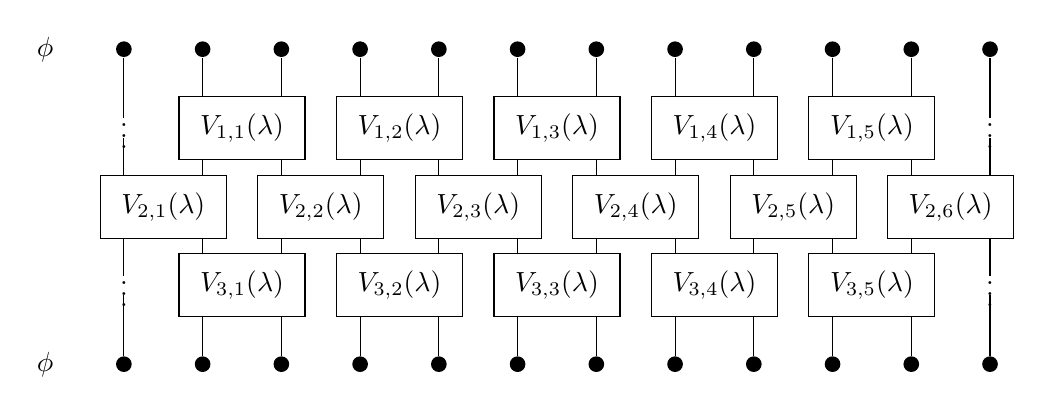
\begin{tikzpicture}
	\foreach \x in {0,...,11}{
		\node (\x) [circle,fill,inner sep=2pt] at (\x,0) {};
		\ifthenelse{\x=0\OR\x=11}{\node (2\x) [] at (\x,-1) {$\vdots$};}{\node (2\x) [] at (\x,-1) {};}
		\node (3\x) [circle,fill,inner sep=2pt] at (\x,-2) {};
		\ifthenelse{\x=0\OR \x=11}{\node (4\x) [] at (\x,-3) {$\vdots$};}{\node (4\x) [] at (\x,-3) {};}
		\node (5\x) [circle,fill,inner sep=2pt] at (\x,-4) {};
	}
	
	\foreach \x in {0,...,11}{
		\draw (\x) -- (2\x);
		\draw (2\x) -- (3\x);
		\draw (3\x) -- (4\x);
		\draw (4\x) -- (5\x);
	}
	
	\foreach \x in {1,...,5}
	\draw [fill=white] (2*\x-0.3-1,-0.6) rectangle (2*\x+0.3,-1.4);
	\foreach \x in {0,...,5}
	\draw [fill=white] (2*\x-0.3,-1.6) rectangle (2*\x+0.3+1,-2.4);
	\foreach \x in {1,...,5}
	\draw [fill=white] (2*\x-0.3-1,-2.6) rectangle (2*\x+0.3,-3.4);
	
	\foreach \x in {1,...,5}
	\node [] at (2*\x-0.5,-1) {$V_{1,\x}(\lambda)$};
	\foreach \x in {0,...,5}
	\node [] at (2*\x+0.5,-2) {$V_{2,\pgfmathtruncatemacro\result{\x+1}\result}(\lambda)$};
	\foreach \x in {1,...,5}
	\node [] at (2*\x-0.5,-3) {$V_{3,\x}(\lambda)$};
	
	\node[] at (-1,0) {$\ket{\phi}$};
	\node[] at (-1,-4) {$\ket{\phi}$};
	
\end{tikzpicture}
	\caption{A graphical depiction of a family of loops generated by a continuous family of FDQC's.}
	\label{fig:FiniteDepthQuantumCirquitLoop}
\end{figure}
As we did before we will sometimes consider the explicit case where the two parameter family, $K(\lambda,s)$, is such that $s\mapsto K(\lambda,s)$ generates a FDQC of depth $D$ for each $\lambda$. We will call this FDQC $V(\lambda)$. We will also ask that we can take each of the local unitaries of $V(\lambda)$ to be continuous in $\lambda$\footnote{This does not immediately follow from the continuity of $K$ itself but it is nevertheless not hard to see that this assumption does not bring much loss of generality.}. A graphical depiction of such a one parameter family of FDQC generated loops is given in \ref{fig:FiniteDepthQuantumCirquitLoop}. Clearly if the $K(\lambda,s)$ contains only $G$-invariant local therms, the local unitaries $V_{i,j}(\lambda)$ will be $G$-invariant as well.
\subsection{Classification of loops: An example}\label{sec:classification-of-loops-an-example}
\subsubsection{Defining the loop}
\begin{figure}
	\centering
	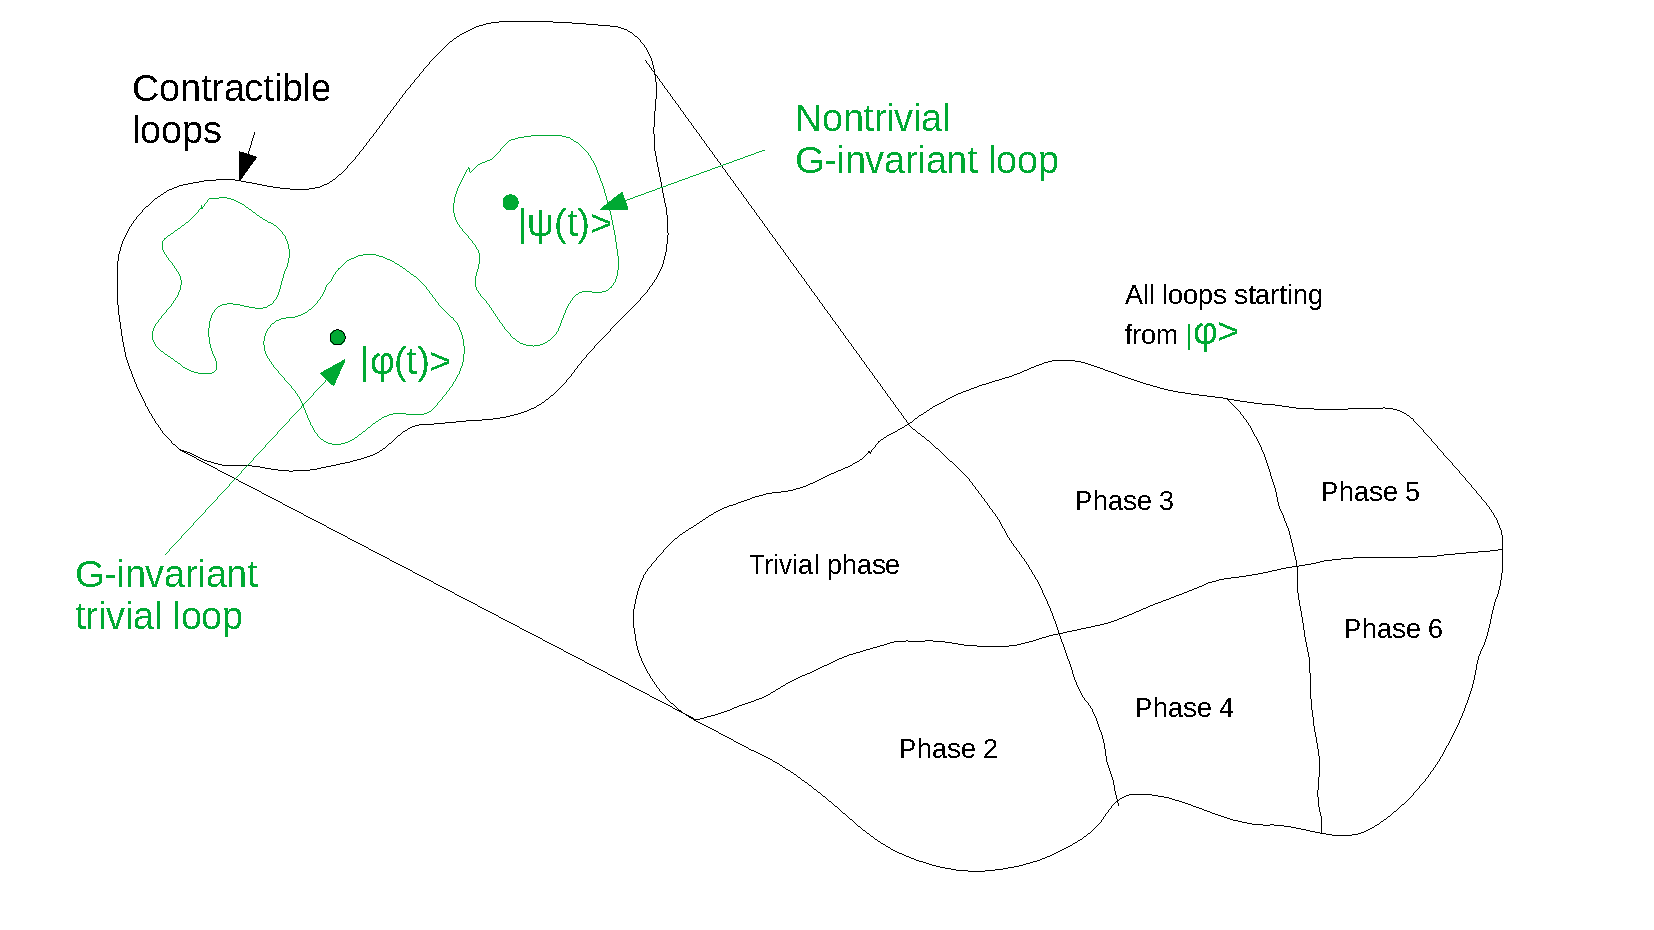
\includegraphics[width=0.8\textwidth]{SPT_Loop_Phases.pdf}
	\caption{This figure shows all loops starting from some $G$-invariant product state (here $\ket{\phi}=\ket{\phi(0)}=\ket{\psi(0)}$). The highlighted black area displays all loops equivalent to the trivial loop (also called contractible loops) while the green areas show the $G$-invariant loops that are $G$-equivalent to each other.}
	\label{fig:ConnectedComponentsLoops}
\end{figure}
\begin{figure}
	\centering
	\scalebox{0.78}{
	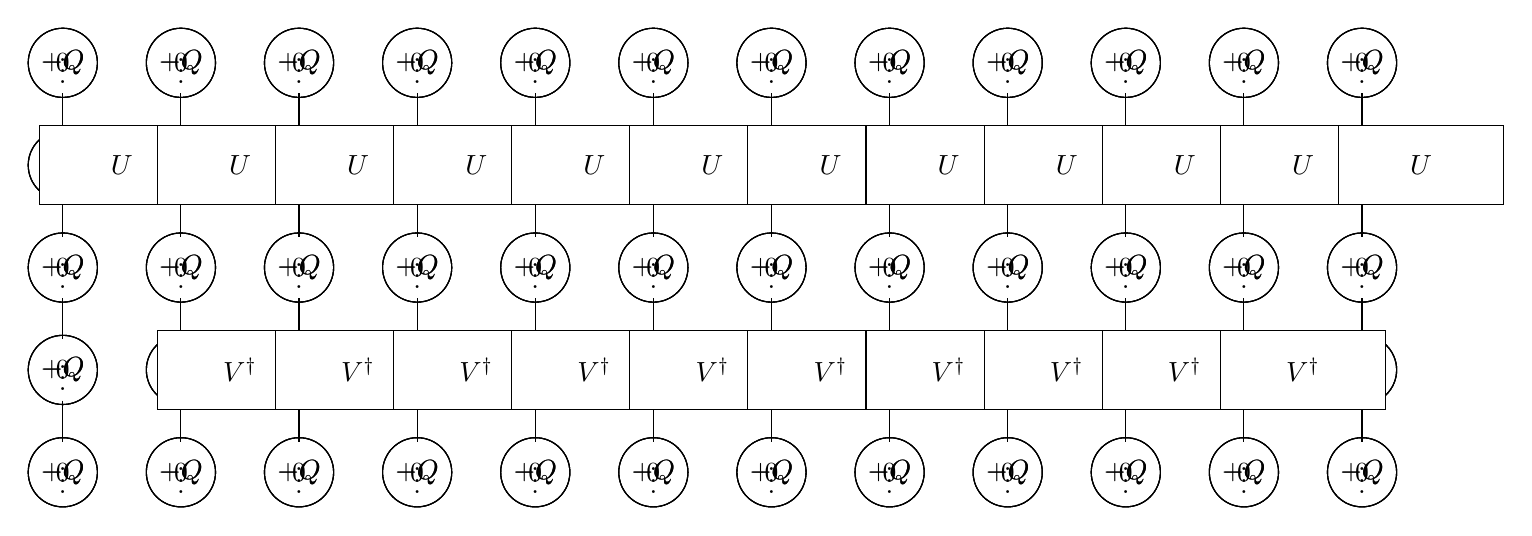
\begin{tikzpicture}
	\newcommand\Distance{1.5}
	\newcommand\yDistance{1.3}
	\newcommand{\NumberOfSites}{11}
	\foreach \x in {0,...,\NumberOfSites}{
		\foreach \y in {0,...,4}{
			\ifthenelse{\y=0\OR\y=4}{\node[circle,draw=black,inner sep=0pt,minimum size=25pt] (\x_\y) at (\Distance*\x,-\yDistance*\y) {$0$};}{
				\ifthenelse{\y=2}{
					\ifthenelse{\isodd{\x}}{\node[circle,draw=black,inner sep=0pt,minimum size=25pt] (\x_\y) at (\Distance*\x,-\yDistance*\y) {$+Q$};}{\node[circle,draw=black,inner sep=0pt,minimum size=25pt] (\x_\y) at (\Distance*\x,-\yDistance*\y) {$-Q$};}}
				{
					\node[] (\x_\y) at (\Distance*\x,-\yDistance*\y) {$\vdots$};
				}
			}
		}
	}
	\foreach \x in {0,...,\NumberOfSites}{
		\foreach \y in {0,...,3}{
			\draw[draw=black] (\x_\y) -- (\x_\the\numexpr \y + 1\relax);
	}}
	\foreach \x in {0,...,\NumberOfSites}{\ifthenelse{\isodd{\x}}{}{
			\draw[fill=white] (\Distance*\x-0.3,-\yDistance*1+0.5) rectangle (\Distance*\x+\Distance+0.3,-\yDistance*1-0.5);
			\node[] (U1_\x) at (\Distance*\x+0.5*\Distance,-\yDistance) {$U$};
	}}
	\foreach \x in {1,...,\the\numexpr \NumberOfSites - 1\relax}{\ifthenelse{\isodd{\x}}{
			\draw[fill=white] (\Distance*\x-0.3,-\yDistance*3+0.5) rectangle (\Distance*\x+\Distance+0.3,-\yDistance*3-0.5);
			\node[] (U2_\x) at (\Distance*\x+0.5*\Distance,-\yDistance*3) {$V^\dagger$};
		}{}}
\end{tikzpicture}
	}
	\caption{This figure displays the FDQC associated to a $U(1)$-invariant loop demonstrating a charge transport $+Q$.}
	\label{fig:U1_ThoulessPumpAs_FiniteDepthQuantumCircuit}
\end{figure}
The goal here is now to do exactly the same thing as we did in the first few sections. We again highlight what we do with a figure (see figure \ref{fig:ConnectedComponentsLoops} which should be seen in contrast to figure \ref{fig:ConnectedComponents}). We first consider all loops starting from some $G$-invariant product state $\ket{\phi}$. We then look at all loops that are equivalent to the trivial loop. We call these loops contractible. Out of all contractible loops, we now look only at the $G$-invariant loops and we group together all $G$-equivalent $G$-invariant loops. These $G$-invariant loops together with this equivalence class is then called the classification of $G$-invariant loops.\\\\
Now it is again time for an example. This example considers loops on the one dimensional lattice (over $\ZZ$). This time we will take as group $U(1)$. We will write the elements of this group as $e^{i\theta}$ where $\theta\in\TT$. Now chose an integer $Q\in\NN$ (we will later on refer to this integer as the charge). We will take as on-site Hilbert space $\CC^3$ and we will label the vectors by $\ket{-Q}$, $\ket{0}$ and $\ket{+Q}.$ Finally we let our on-site group action $U(\theta)$ be such that
\begin{align}
	U(\theta)\ket{-Q}&=e^{-i Q\theta}\ket{-Q}&U(\theta)\ket{0}&=\ket{0}&U(\theta)\ket{+Q}&=e^{+iQ\theta}\ket{+Q}.
\end{align}
Now I will define a $G$-invariant loop starting from the product state
\begin{equation}
	\ket{\phi}=\bigotimes_{i\in\Lambda}\ket{0}.
\end{equation}
To do this, let $U=\exp(-iK_1)$ and let $V=\exp(-i K_2)$ where
\begin{align}
	K_1&=i(\ket{0,0}\bra{-Q,+Q}-\ket{-Q,+Q}\bra{0,0})&K_2&=i(\ket{0,0}\bra{+Q,-Q}-\ket{+Q,-Q}\bra{0,0}).
\end{align}
Since $K_1$ and $K_2$ are hermitian, these are unitary operators. Furthermore, since $K_1$ and $K_2$ are $G$-invariant, they are $G$-invariant unitaries. A quick calculation shows that
\begin{align}
	U\ket{0,0}&=\ket{-Q,+Q}&V \ket{0,0}&=\ket{+Q,-Q}.
\end{align}
We can now use these unitaries to create a $G$-invariant depth 2 quantum cirquit. We use $U$ to create the first layer and $V$ to create the second layer. The full finite depth quantum cirquit is then given by
\begin{equation}
	W=\bigotimes_{i\in\Lambda_{\text{odd}}}V_{i,i+1}\bigotimes_{i\in\Lambda_{\text{even}}}U_{i,i+1}.
\end{equation}
See figure \ref{fig:U1_ThoulessPumpAs_FiniteDepthQuantumCircuit} for a graphical depiction of this FDQC.
\begin{figure}
	\centering
	\scalebox{0.78}{
		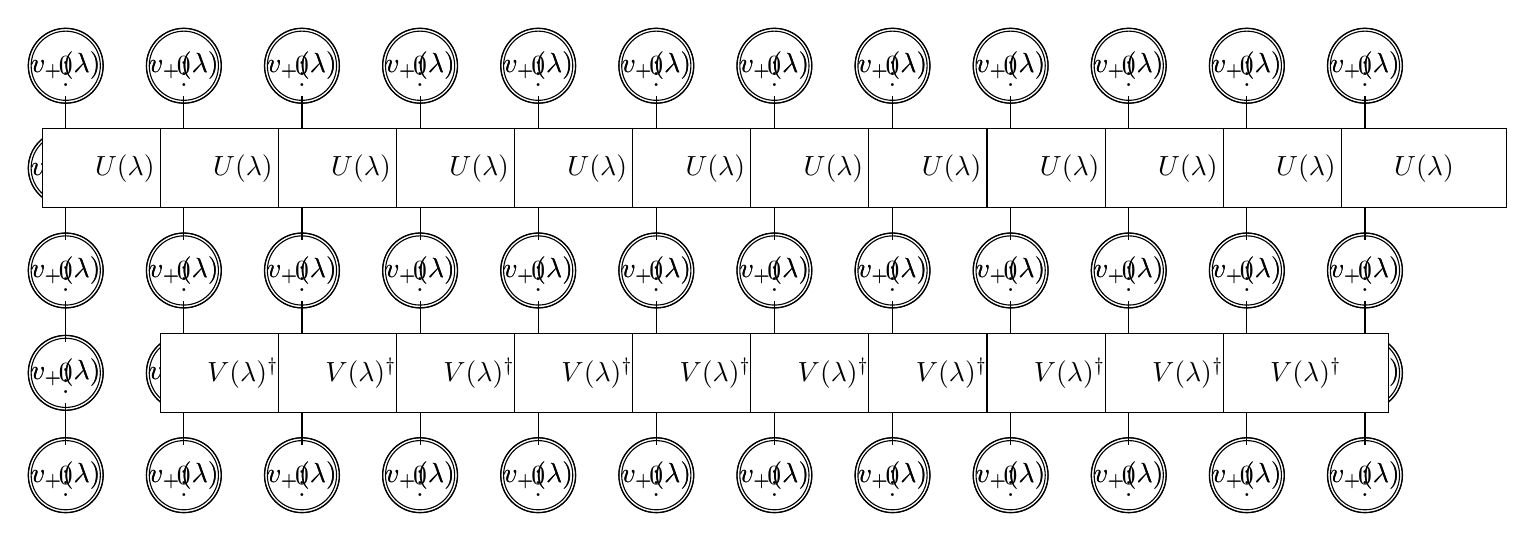
\begin{tikzpicture}
	\newcommand\Distance{1.5}
	\newcommand\yDistance{1.3}
	\newcommand{\NumberOfSites}{11}
	\foreach \x in {0,...,\NumberOfSites}{
		\foreach \y in {0,...,4}{
			\ifthenelse{\y=0\OR\y=4}{\node[circle,draw=black,inner sep=0pt,minimum size=25pt] (\x_\y) at (\Distance*\x,-\yDistance*\y) {$0$};}{
				\ifthenelse{\y=2}{
					\ifthenelse{\isodd{\x}}{\node[circle,draw=black,inner sep=0pt,minimum size=25pt] (\x_\y) at (\Distance*\x,-\yDistance*\y) {$v_+(\lambda)$};}{\node[circle,draw=black,inner sep=0pt,minimum size=25pt] (\x_\y) at (\Distance*\x,-\yDistance*\y) {$v_-(\lambda)$};}}
				{
					\node[] (\x_\y) at (\Distance*\x,-\yDistance*\y) {$\vdots$};
				}
			}
		}
	}
	\foreach \x in {0,...,\NumberOfSites}{
		\foreach \y in {0,...,3}{
			\draw[draw=black] (\x_\y) -- (\x_\the\numexpr \y + 1\relax);
	}}
	\foreach \x in {0,...,\NumberOfSites}{\ifthenelse{\isodd{\x}}{}{
			\draw[fill=white] (\Distance*\x-0.3,-\yDistance*1+0.5) rectangle (\Distance*\x+\Distance+0.3,-\yDistance*1-0.5);
			\node[] (U1_\x) at (\Distance*\x+0.5*\Distance,-\yDistance) {$U(\lambda)$};
	}}
	\foreach \x in {1,...,\the\numexpr \NumberOfSites - 1\relax}{\ifthenelse{\isodd{\x}}{
			\draw[fill=white] (\Distance*\x-0.3,-\yDistance*3+0.5) rectangle (\Distance*\x+\Distance+0.3,-\yDistance*3-0.5);
			\node[] (U2_\x) at (\Distance*\x+0.5*\Distance,-\yDistance*3) {$V(\lambda)^\dagger$};
		}{}}
\end{tikzpicture}
	}
	\caption{This figure displays the (non $G$-invariant) contraction of the loop displayed in figure \ref{fig:U1_ThoulessPumpAs_FiniteDepthQuantumCircuit}.}
	\label{fig:U1_ThoulessPumpAs_FiniteDepthQuantumCircuit_Contraction}
\end{figure}
\subsubsection{Non $G$-invariant contraction}
Now I will show That this loop is contractible in a non $G$-invariant way. To this end, define the one parameter family of vectors
\begin{align}
	v_-(\lambda)&=\sin(2\pi\lambda)\ket{-Q}+\cos(2\pi\lambda)\ket{0}&v_+(\lambda)&=\sin(2\pi\lambda)\ket{+Q}+\cos(2\pi\lambda)\ket{0}.
\end{align}
Similarly to our original loop we now let $U(\lambda)=\exp(-iK_1(\lambda))$ and let $V(\lambda)=\exp(-i K_2(\lambda))$ where
\begin{align}
	K_1(\lambda)&=i(\ket{0,0}\bra{v_-(\lambda),v_+(\lambda)}-\ket{v_-(\lambda),v_+(\lambda)}\bra{0,0})\\
	K_2(\lambda)&=i(\ket{0,0}\bra{v_+(\lambda),v_-(\lambda)}-\ket{v_+(\lambda),v_-(\lambda)}\bra{0,0}).
\end{align}
These will indeed satisfy that $U(0)=V(0)=\id_{\CC^3}$, $U(1)=U$ and $V(1)=V$. Moreover if you create the same depth 2 quantum cirquit you will still create a loop (as is displayed in figure \ref{fig:U1_ThoulessPumpAs_FiniteDepthQuantumCircuit_Contraction}).
\subsection{The boundary state}
\begin{figure}
	\centering
	\scalebox{0.6}{
		\begin{tikzpicture}
\newcommand{\Dx}{1}
\newcommand{\Dy}{1}
\newcommand{\TotalSites}{19}
\node[] (FirstState) at (-2,0) {$\begin{matrix}
		\ket{\phi}=\\\ket{\phi_L}\otimes\ket{\phi_C}\otimes\ket{\phi_R}
	\end{matrix}$};
\node[] (LastState) at (-2,-6) {$\begin{matrix}
		\ket{\tilde{\phi}(\lambda)}=\\ \ket{\phi_L}\otimes\ket{\psi(\lambda)}\otimes\ket{\phi_R}
	\end{matrix}$};
\foreach \x in {0,...,\TotalSites}{
	\foreach \y in {0,...,6}{
		\ifthenelse{\y=0\OR\y=6}{\node (\x_\y) [circle,fill,inner sep=2pt] at (\Dx*\x,-\Dy*\y) {};}{
			\ifthenelse{\NOT\(\isodd{\y}\)\AND\(\x=0\OR\x=\TotalSites\)}{\node (\x_\y) [] at (\Dx*\x,-\Dy*\y) {$\vdots$};}{\node (\x_\y) [] at (\Dx*\x,-\Dy*\y) {};}
		}
	}
}
\foreach \x in {0,...,\TotalSites}{
	\foreach \y in {0,...,6}{
		\newcommand{\yplus}{\the\numexpr\y+1\relax}
		\ifthenelse{\y=6}{}{\draw (\x_\y)--(\x_\yplus);}
	}
}
\foreach \x in {0,...,\TotalSites}{
	\foreach \y in {1,...,5}{
		\ifthenelse{\isodd{\y}}{
			\ifthenelse{\isodd{\x}}{}{
				\ifthenelse{\(\y=1\AND\x=8\)\OR\(\y=3\AND\(\x=8\OR\x=10\)\)\OR\(\y=5\AND\(\x=8\OR\x=10\OR\x=12\)\)}{\draw[fill=yellow] (\Dx*\x-\Dx*0.3,-\Dy*\y+\Dy*0.3) rectangle (\Dx*\x+\Dx*1.3,-\Dy*\y-\Dy*0.3);
				\node[] (V_\x_\y) at (\Dx*\x+0.5\Dx,-\Dy*\y) {$V_{\y,\the\numexpr\x/2\relax}(\lambda)$};
				}{\draw[fill=white] (\Dx*\x-\Dx*0.3,-\Dy*\y+\Dy*0.3) rectangle (\Dx*\x+\Dx*1.3,-\Dy*\y-\Dy*0.3);
				\node[] (V_\x_\y) at (\Dx*\x+0.5\Dx,-\Dy*\y) {$V_{\y,\the\numexpr\x/2\relax}(\lambda)$};
				}
				
				\ifthenelse{\x<10.5}{\draw (\Dx*\x-\Dx*0.3,-\Dy*\y+\Dy*0.4)--(\Dx*\x+\Dx*1.3,-\Dy*\y-\Dy*0.4);}{}
			}
		}{
			\ifthenelse{\isodd{\x}\AND\(\NOT\(\x=\TotalSites\)\)}{
				\ifthenelse{\(\y=2\AND\x=9\)\OR\(\y=4\AND\(\x=9\OR\x=11\)\)}{\draw[fill=yellow] (\Dx*\x-\Dx*0.3,-\Dy*\y+\Dy*0.3) rectangle (\Dx*\x+\Dx*1.3,-\Dy*\y-\Dy*0.3);
				\node[] (V_\x_\y) at (\Dx*\x+0.5\Dx,-\Dy*\y) {$V_{\y,\the\numexpr\x/2\relax}(\lambda)$};
				}{\draw[fill=white] (\Dx*\x-\Dx*0.3,-\Dy*\y+\Dy*0.3) rectangle (\Dx*\x+\Dx*1.3,-\Dy*\y-\Dy*0.3);
				\node[] (V_\x_\y) at (\Dx*\x+0.5\Dx,-\Dy*\y) {$V_{\y,\the\numexpr\x/2\relax}(\lambda)$};
				}
				
				\ifthenelse{\x<10.5}{\draw (\Dx*\x-\Dx*0.3,-\Dy*\y+\Dy*0.4)--(\Dx*\x+\Dx*1.3,-\Dy*\y-\Dy*0.4);}{}}{}
		}
	}
}
\draw (\Dx*\TotalSites/2,\Dy*0.5)--(\Dx*\TotalSites/2,-\Dy*6-\Dy*0.5);
\draw [decorate,decoration={brace,amplitude=5pt},xshift=0cm,yshift=0pt] (\Dx*9.5,-\Dy*6-0.1*\Dy) -- (0,-\Dy*6-0.1*\Dy) node [black,midway,yshift=-0.5cm] {$\AA_L$};
\draw [decorate,decoration={brace,amplitude=5pt},xshift=0cm,yshift=0pt] (\Dx*13.5,-\Dy*6-0.1*\Dy) -- (\Dx*9.5,-\Dy*6-0.1*\Dy) node [black,midway,yshift=-0.5cm] {$\AA_C$};
\draw [decorate,decoration={brace,amplitude=5pt},xshift=0cm,yshift=0pt] (\Dx*\TotalSites,-\Dy*6-0.1*\Dy)-- (\Dx*13.5,-\Dy*6-0.1*\Dy) node [black,midway,yshift=-0.5cm] {$\AA_R$};
\end{tikzpicture}
	}
	\caption{A graphical depiction of the action of the FDQC $\tilde{V}(\lambda)$ on the product state $\ket{\phi}$. The state $\ket{\psi(\lambda)}$ is the boundary state of the loop and is continuous in $\lambda$.}
	\label{fig:G_InvariantContraction_WithLightcone}
\end{figure}
One property that any loop (on any lattice) has is that it has an associated boundary state. In this section we will construct this boundary state and describe some of its properties. As was the case before, all the pictures I make in this section will be on the one dimensional lattice but can be generalised in a straightforward way to higher dimensions.\\\\
Suppose that the loop is generated by some depth-D FDQC $V$. Define $\tilde{V}$ that is constructed by taking all local unitaries of $V$ that have support on the right of the origin and setting all others to $0$ (see figure \ref{fig:G_InvariantContraction_WithLightcone}). Let $\ket{\tilde{\phi}}\defeq \tilde{V}\ket{\phi}$. Take the three local algebras, $\AA_L$, $\AA_C$ and $\AA_R$ as shown in figure \ref{fig:G_InvariantContraction_WithLightcone}. We now get that for any $a\in \AA_L$ and any $b\in\AA_R$
\begin{align}
	\bra{\tilde{\phi}}a\ket{\tilde{\phi}}&=\bra{\phi_L}a\ket{\phi_L}&\bra{\tilde{\phi}}b\ket{\tilde{\phi}}&=\bra{\phi_R}b\ket{\phi_R}.
\end{align}
This implies that there must exist a state $\ket{\psi}$ such that
\begin{equation}
	\ket{\tilde{\phi}}=\ket{\phi_L}\otimes\ket{\psi}\otimes\ket{\phi_R}.
\end{equation}
We call this state $\ket{\psi}$, the boundary state of $(V,\ket{\phi})$. Some remarks here:
\begin{enumerate}
	\item If each layer of the loop is $G$-invariant it is easy to see that that the boundary state will be $G$-invariant.
	\item If we have two equivalent loops then their boundary states have to be equivalent as 0-dimensional states.
	\item If we have two $G$-equivalent loops then their boundary states have to be equivalent as $G$-invariant, 0-dimensional states.
	\item In principle, we can define this boundary state also for any lattice of the form $\ZZ^d$ for any positive integer $d$. The boundary state will then be a state over the lattice $\ZZ^{d-1}$. However ,the last statement that an equivalence of loops implies an equivalence of states is not so trivial any more. The statement is still believed to be true {\color{red}citation needed?}.
\end{enumerate}

\subsection{No $G$-invariant contraction}
\begin{figure}
	\centering
	\scalebox{0.8}{
	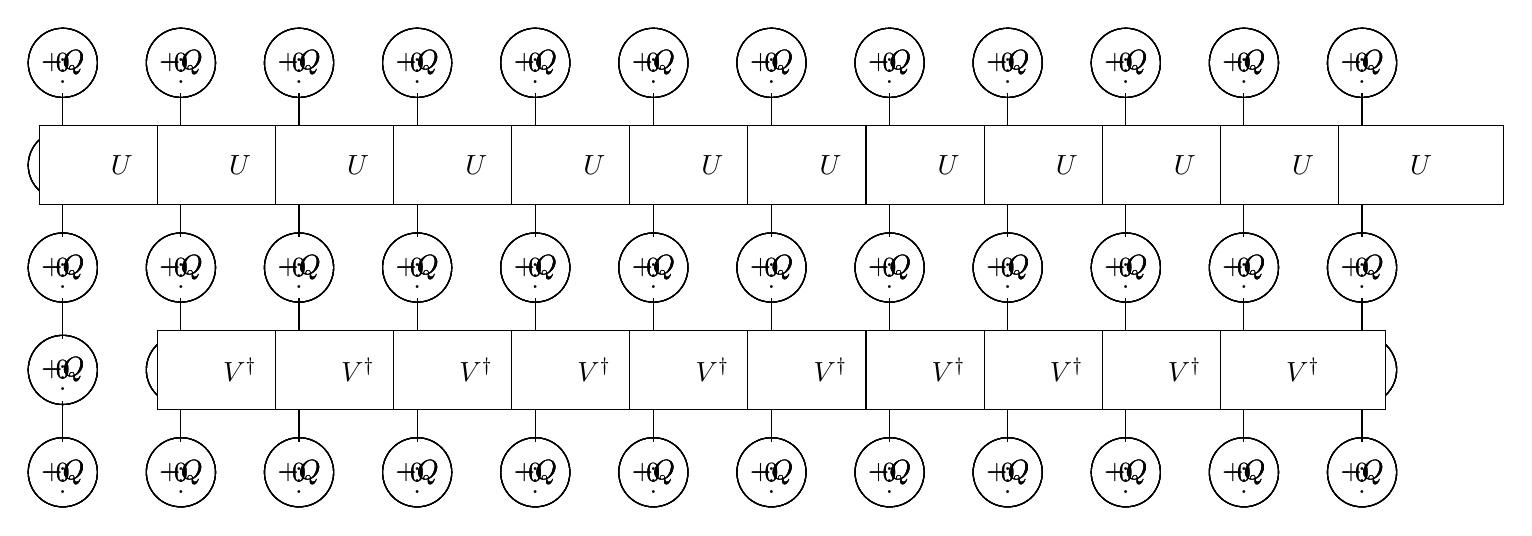
\begin{tikzpicture}
	\newcommand\Distance{1.5}
	\newcommand\yDistance{1.3}
	\newcommand{\NumberOfSites}{11}
	\foreach \x in {0,...,\NumberOfSites}{
		\foreach \y in {0,...,4}{
			\ifthenelse{\y=0\OR\y=4}{
				\ifthenelse{\y=4\AND\x=6}{\node[circle,draw=black,inner sep=0pt,minimum size=25pt] (\x_\y) at (\Distance*\x,-\yDistance*\y) {$-Q$};}{\node[circle,draw=black,inner sep=0pt,minimum size=25pt] (\x_\y) at (\Distance*\x,-\yDistance*\y) {$0$};}
				
				}{
				\ifthenelse{\y=2}{
					\ifthenelse{\x<6}{\node[circle,draw=black,inner sep=0pt,minimum size=25pt] (\x_\y) at (\Distance*\x,-\yDistance*\y) {$0$};}{
					\ifthenelse{\isodd{\x}}{\node[circle,draw=black,inner sep=0pt,minimum size=25pt] (\x_\y) at (\Distance*\x,-\yDistance*\y) {$+Q$};}{\node[circle,draw=black,inner sep=0pt,minimum size=25pt] (\x_\y) at (\Distance*\x,-\yDistance*\y) {$-Q$};}}}
				{
					\node[] (\x_\y) at (\Distance*\x,-\yDistance*\y) {$\vdots$};
				}
			}
		}
	}
	\foreach \x in {0,...,\NumberOfSites}{
		\foreach \y in {0,...,3}{
			\draw[draw=black] (\x_\y) -- (\x_\the\numexpr \y + 1\relax);
	}}
	\foreach \x in {0,...,\NumberOfSites}{\ifthenelse{\isodd{\x}}{}{
			\draw[fill=white] (\Distance*\x-0.3,-\yDistance*1+0.5) rectangle (\Distance*\x+\Distance+0.3,-\yDistance*1-0.5);
			
			\ifthenelse{\x<5}{\node[] (U1_\x) at (\Distance*\x+0.5*\Distance,-\yDistance) {$\id$};}{\node[] (U1_\x) at (\Distance*\x+0.5*\Distance,-\yDistance) {$U$};}
	}}
	\foreach \x in {1,...,\the\numexpr \NumberOfSites - 1\relax}{\ifthenelse{\isodd{\x}}{
			\draw[fill=white] (\Distance*\x-0.3,-\yDistance*3+0.5) rectangle (\Distance*\x+\Distance+0.3,-\yDistance*3-0.5);
			\ifthenelse{\x<6}{\node[] (U2_\x) at (\Distance*\x+0.5*\Distance,-\yDistance*3) {$\id$};}{\node[] (U2_\x) at (\Distance*\x+0.5*\Distance,-\yDistance*3) {$V^\dagger$};}
			
		}{}}
\end{tikzpicture}
	}
	\caption{}
	\label{fig:U1_ThoulessPumpAs_FiniteDepthQuantumCircuit_Boundary}
\end{figure}
Now we will show that the $G$-invariant loop presented in section \ref{sec:classification-of-loops-an-example} cannot have a $G$-invariant contraction. To see this, we first create the boundary state of this loop. This is done in figure \ref{fig:U1_ThoulessPumpAs_FiniteDepthQuantumCircuit_Boundary}. It creates a 0-dimensional SPT state with charge $-Q$.\\\\
Now, suppose there was a family of depth-D FDQCs, $V(\lambda)$ such that $V(0)=\id$ and $V(1)$ generates the loop given in section \ref{sec:classification-of-loops-an-example}. Let $\ket{\psi(\lambda)}$ be the boundary state of $(V(\lambda),\ket{\phi})$. It has to be a continuous family of states connecting the boundary state of $(V,\ket{\phi})$ to the $G$-invariant product state that is the boundary state of $(\id,\ket{\phi})$. Since the boundary state of $(V,\ket{\phi})$ had charge $-Q$ and the boundary state of $(\id,\ket{\phi})$ has charge $0$, this is not possible. This shows that there does not exist a contraction.\\\\
This allows us to come to the following conjecture that we will prove in chapter {\color{red}reference needed} of this thesis:
\begin{conjecture}
	The classification of $G$-invariant loops is fully determined by the classification of their respective boundary states.
\end{conjecture}
\section{Space groups}
In the last sections we have looked at the classifications of SPT states and Loops of SPT states respectively. In both of these cases the symmetry was an on-site symmetry. In this section we will generalize this assumption and include some other symmetries. We will here ask the question, what if the group action isn't even a finite depth quantum cirquit.
\subsection{Translations}
\begin{figure}
	\scalebox{0.7}{
	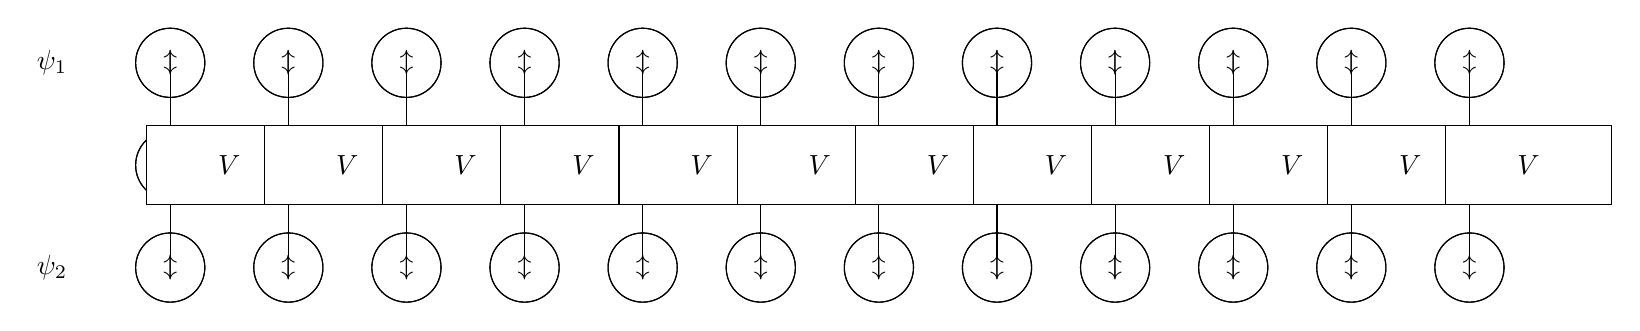
\begin{tikzpicture}
	\newcommand\Distance{1.5}
	\newcommand\yDistance{1.3}
	\newcommand{\NumberOfSites}{11}
	\foreach \x in {0,...,\NumberOfSites}{
		\foreach \y in {0,...,2}{
			\ifthenelse{\y=0}{\node[circle,draw=black,inner sep=0pt,minimum size=25pt] (\x_\y) at (\Distance*\x,-\yDistance*\y) {$\uparrow$};}{
				\ifthenelse{\y=2}{\node[circle,draw=black,inner sep=0pt,minimum size=25pt] (\x_\y) at (\Distance*\x,-\yDistance*\y) {$\downarrow$};}{\node[] (\x_\y) at (\Distance*\x,-\yDistance*\y) {};}}
			}
	}
	\node[] (Psi1) at (-\Distance,0) {$\ket{\psi_1}$};
	\node[] (Psi2) at (-\Distance,-2*\yDistance) {$\ket{\psi_2}$};
	\foreach \x in {0,...,\NumberOfSites}{
		\foreach \y in {0,...,1}{
			\draw[draw=black] (\x_\y) -- (\x_\the\numexpr \y + 1\relax);
	}}
	\foreach \x in {0,...,\NumberOfSites}{\ifthenelse{\isodd{\x}}{}{
			\draw[fill=white] (\Distance*\x-0.3,-\yDistance*1+0.5) rectangle (\Distance*\x+\Distance+0.3,-\yDistance*1-0.5);
			\node[] (U1_\x) at (\Distance*\x+0.5*\Distance,-\yDistance) {$V$};
	}}
\end{tikzpicture}
	}
	\caption{This is a $G$-invariant finite depth quantum cirquit. It is however not translation invariant (Not over one site at least. It is translation invariant over two sites).}
	\label{fig:Z_2_and_TranslationInvariantStates}
\end{figure}
The translation is an automorphism, $\tau$ that takes an element of the operator algebra and shifts its support by one site. A state will be called translation invariant if its expectation value with respect to any translated operator is equal to the original expectation value. More specifically, $\ket{\psi}$ is translation invariant if
\begin{equation}
	\bra{\psi}A\ket{\psi}=\bra{\psi}\tau(A)\ket{\psi}
\end{equation}
for all $A\in\AA$. Just like was the case with loops we won't merely look at states that are translation invariant but specifically at $G$-invariant states that are also translation invariant. This end we ask that our on site group action is translation invariant (we associate to each site the same representation).\\\\
We now have to explain what it means for a LGU to be translation invariant. As mentioned before $V(t)$ was an LGU if there is a one parameter family of Hermitian sum of local therms operators $K(s)$ such that
\begin{equation}
	V(t)=\mathcal{T}\exp(-i\int_{0}^{t}\d s K(s)).
\end{equation}
Now lets make a choice for these local therms, namely we take $K_i(s)$, one parameter families of Hermitian operators. We say that $K(s)$ with this choice of decomposition is translation invariant if for each $i$ there exists a $j$ such that
\begin{equation}
	\tau(K_i(s))=K_j(s).
\end{equation}
This should be seen in contrast with the on-site group action where we had that $K(s)$ with this choice of decomposition is $G$-invariant if
\begin{equation}
	\Ad{U(g)}(K_i(s))=K_i(s).
\end{equation}
The main question we will be asking in this section is now the following:
\begin{itemize}
	\item Let $\ket{\psi_1}$ and $\ket{\psi_2}$ be two translation invariant, $G$-invariant SPT's. Suppose there exists a $G$-invariant LGU connecting $\ket{\psi_1}$ and $\ket{\psi_2}$, does this imply there exists an LGU that is both $G$-invariant and translation invariant that does this? If this does not exist then what is the obstruction to finding this?
\end{itemize}
As an example, consider $G=\ZZ_2$. We will denote the elements of $\ZZ_2$ with multiplicative notation as $1$ and $-1$. We let this group act on the on-site Hilbert space $\CC^2$ through
\begin{align}
	U(1)\ket{\uparrow}&=\ket{\uparrow}&U(1)\ket{\downarrow}&=\ket{\downarrow}\\
	U(-1)\ket{\uparrow}&=\ket{\uparrow}&U(-1)\ket{\downarrow}&=-\ket{\downarrow}.
\end{align}
The two examples of translation invariant $G$-invariant states that we will consider are the product state with $\ket{\uparrow}$ vectors everywhere which we will call $\ket{\psi_1}$ and the product state with $\ket{\downarrow}$ vectors everywhere which we will call $\ket{\psi_2}$. As is depicted in figure \ref{fig:Z_2_and_TranslationInvariantStates}, these two states can indeed be deformed into one another via a $G$-invariant LGU. Can I find a $G$-invariant LGU that is translation invariant as well? It turns out that the answer to this question is no. The reason why this is the case is that in chapter {\color{red}reference} we provide an $H^1(G,\TT)-$valued index for any $G$-invariant, translation invariant state that is invariant under applying $G$-invariant, translation invariant LGU's. If one combines the translation index with the SPT index mentioned previously, one obtains an $H^2(G,\TT)\oplus H^1(G,\TT)$-valued index.
\subsection{Mirror symmetry}
Previously every additional symmetry we imposed just resulted in another index for the classification problem. This seems to be the case for every symmetry that preserves the orientation of the lattice\footnote{I am only talking about the lattices $\ZZ^d$ for which there are no difficulties to defining an orientation}. It turns out however that orientation reversing symmetries can restrict some of the previous indices. By this I mean that the cochains that are used to define the SPT index have to satisfy some additional property. This reduces the amount of SPT classes one can get.\\\\
Remember that we previously classified $G$-symmetric SPT's over the lattice $\ZZ$ by looking at the cochains corresponding to projective representations. We did this by looking at how the state transforms under the group action on the right half of the lattice. Say that the right half of the chain transforms under some projective representation $U_R(g)$. We can do the same with the left half of the chain. Say we call this projective representation $U_L(g)$. Since the full state is $G$-invariant, we require
\begin{equation}
	U(g)=U_L(g)\otimes U_R(g)
\end{equation}
to be a linear representation. It turns out ({\color{red}I have to explain this further}) that if our state is translation invariant there is a unitary, $V$ such that
\begin{equation}
	U_L(g)=V^\dagger U_R(g)V.
\end{equation}
Now let $C:G^2\rightarrow U(1)$ be the 2-cochain such that
\begin{equation}
	U_R(g)U_R(h)=C(g,h)U_R(gh)
\end{equation}
then we require that
\begin{equation}
	C(g,h)^2=0.
\end{equation}
This means that the amount of $G$-invariant SPT's over $\ZZ$ that are mirror symmetric are partially\footnote{The full index for $G$-invariant SPT's that are mirror symmetric is $\ZZ_2\oplus H^1(G,\TT)\oplus (\ZZ_2\otimes H^2(G,\TT))$.} classified by
\begin{equation}
	\ZZ_2\otimes H^2(G,\TT).
\end{equation}
\section{Tools for quantum many body physics}
\label{sec:ToolsForQuantumManyBody}
In the last few sections I have made statements like: "the right half part of this states transforms under a projective representation" or "the restriction to the right of the loop operator applied on the product state creates a zero dimensional SPT". With both statements is one common flaw though. These statements where meant for the situation where the lattice is $\ZZ$ but in this case there is no notion of a full Hilbert space. Both for defining representations and for defining zero dimensional SPT states I need a Hilbert space. This begs the question, on what Hilbert space is this true. Similar problems can be found with the sum of local therms operators introduced in the beginning (see for example the $K$ in definition \ref{def:ConnectedStates}). If the lattice is non-compact, there is no reason for the sum over the local therms to be convergent.\\\\
In this section we will develop some definitions and mathematical tools that are most frequently used in this thesis. They are used to address some of these issues as well as allowing us to generalise some of our previously made statements.
\subsection{The quasi local $C^*$-algebra}
First we define the operator algebra we will be working on. To do this, we first choose a lattice. This is a discrete set, $\Gamma$ with some notion of distance on it which we will denote by $d:\Gamma^2\rightarrow \RR$. In this thesis we will mainly be working with three lattices. That is, the lattice with one point ($\ZZ_1$), the one dimensional lattice ($\ZZ$) and the two dimensional lattice ($\ZZ^2$).\\\\
Next we must create the operator algebra. This will be very similar to what we did in figure \ref{fig:Lattice}. We first fix an on site Hilbert space. As we did before, we can still simply take $\CC^d$ for some integer $d\in\NN$ (where $d$ could possibly depend on the site). Next we define the local algebra. To this end, let $\mathfrak{B}_{\Gamma}$. For any $\Lambda\in\mathfrak{B}_\Gamma$ we define the algebra over $\Lambda$ through:
\begin{equation}
	\AA_{\Lambda}=\bigotimes_{i\in\Lambda}\BB(\CC^d).
\end{equation}
We define this algebra in such a way that the inclusion on $\mathfrak{B}_\Gamma$ define an embedding on the algebra
\begin{align}
	\Lambda_1&\subset\Lambda_2&&\Rightarrow&\AA_{\Lambda_1}&\subset\AA_{\Lambda_2}.
\end{align}
This embedding is defined by mapping $a\in\AA_{\Lambda_1}$ to $\left(\bigotimes_{i\in\Lambda_2\backslash\Lambda_1}\id_{\CC^d}\right)\otimes a\in \AA_{\Lambda_2}$. If we now define the local algebra by taking the union over all finite sets
\begin{equation}
	\AA_{\text{loc}}=\bigcup_{\Lambda\in\mathfrak{B}_\Gamma}\AA_\Lambda
\end{equation}
and by identifying any two operators that can be embedded into the same operator (in some bigger still finite subset of $\Gamma$). One can easily check that this is indeed a well defined algebra. Now, let $\norm{\cdot}$ be the operator norm on the (tensor products of) the on site Hilbert spaces. This norm is indeed invariant under the choice of embedding. The closure of the local algebra under this norm,
\begin{equation}
	\AA=\overline{\AA_{\text{loc}}}
\end{equation}
is called the quasi-local $C^*$-algebra\footnote{More generally $C^*$-algebras are just Banach algebras (with a norm) and an adjoint but all the $C^*$ algebras considered in this thesis will either be bounded operators on some separable Hilbert space or quasi-local $C^*$ algebras on some lattice.}.
\subsection{The on site group action}
The definition of the on-site group action is again very similar to what we did in section \ref{sec:enriching-the-trivial-phase-with-symmetry} (see figure \ref{fig:GroupActionQuantumCirquit} in particular). We define a group homomorphism on the on-site Hilbert space $U_i\in\hom(G,U(\CC^d))$. In this case however there is no full Hilbert space and therefore, there is no unitary representation of the full group action. It is however very easy to define the adjoint group action on any local operator. Indeed, let $A\in\AA_{\text{loc}}$ be an operator with support in some finite set $\Lambda\in\mathfrak{B}_{\Gamma}$ then we can define
\begin{equation}
	\beta^\Lambda_{g}(A)=\Ad{\bigotimes_{i\in\Lambda}U_i(g)}(A).
\end{equation}
It turns out that this automorphism on the algebra of local operators can be extended to the full quasi local $C^*$-algebra $\AA=\overline{\AA_{\text{loc}}}$. {\color{red}More explanation needed?}
\subsection{Interactions and locally generated automorphisms}
Given a quasi local $C^*$-algebra $\AA$ over a lattice $\Gamma$ with some distance measure $d$ defined on it, an interaction $\Phi$ is a map
\begin{equation}
	\Phi: \mathfrak{G}_{\Gamma}\rightarrow \AA_{\text{loc}}: I \mapsto \Phi(I)
\end{equation}
where $\Phi(I)\in\AA_I$ is hermitian ($\Phi(I)=\Phi(I)^*$).We will sometimes use the restriction of an interaction. For some $\tilde\Gamma\subset\Gamma$ we define $\Phi_{\tilde\Gamma}$ by
\begin{equation}
	\Phi_{\tilde\Gamma}:\mathfrak{G}_{\ZZ^2}\rightarrow \AA_{\text{loc}}:I\mapsto\left\{\begin{matrix}
		\Phi(I)&\text{if }I\subset\Gamma\\0&\text{otherwise}.
	\end{matrix}\right.
\end{equation}
We will sometimes require a norm on the space of interactions that indicates how local an interaction acts. The norm we will used is sometimes called the $F$-norm. It is labeled by some non-increasing positive function $F:\NN\rightarrow \RR^+$. Following \cite{doi:10.1063/1.5095769} we call such a function an $F$-function if it satisfies two conditions:
\begin{enumerate}
	\item $F$ is uniformly integrable over $\Gamma$:
	\begin{equation}\label{eq:F_Is_Uniformly_Integrable_Over_Gamma}
		\norm{F}=\sup_{x\in\Gamma}\sum_{y\in\Gamma}F(d(x,y))<\infty.
	\end{equation}
	\item $F$ satisfies the convolution condition
	\begin{equation}
		\sum_{z\in\Gamma}F(d(x,z))F(d(z,y))< C_F F(d(x,y))
	\end{equation}
	for some finite constant $C_F$.
\end{enumerate}
Given such an $F$-function, we can define a norm on these interactions called 
\begin{equation}
	\norm{\Phi}_F\defeq \sup_{x,y\in\ZZ^2}\frac{1}{F(\abs{x-y})}\sum_{Z\in\mathfrak{G}_{\ZZ^2},Z\ni x,y}\norm{\Phi(Z)}.
\end{equation}
The set of interactions with this norm (for a fixed $F$) is a Banach space. Following \cite{ogata2021h3gmathbb} we will fix a specific family of $F$-functions for the case where $\Gamma=\ZZ^2$. For any $0<\phi<1$ we define
\begin{equation}\label{eq:OurFFunction}
	F_\phi:\RR^+\rightarrow\RR^+:r\mapsto \frac{\exp(-r^\phi)}{(1+r)^4}.
\end{equation}
One of the properties of $F$-local interactions is that they can be used to generate automorphisms. Let
\begin{equation}
	\Phi:\mathfrak{G}_{\Gamma}\times [0,1]\rightarrow \AA_{\text{loc}}:(I,t)\mapsto \Phi(I,t)
\end{equation}
be a piecewise norm continuous\footnote{By which we mean that $\Phi(I,\cdot)$ is piecewise norm continuous for each $I\in\mathfrak{G}_{\ZZ^2}$.} one parameter family of interactions such that the $F$-norm is uniformly bounded ($\sup_{t\in[0,1]}\norm{\Phi(\cdot,t)}_F<\infty$). We will denote the set of one parameter families of interactions that satisfy this property by $\BB_{F}([0,1])$. For any $\Phi\in\BB_{F_\phi}([0,1])$, we define the locally generated automorphism (LGA) $\gamma^{\Phi}_{s;t}$ such that for any $A\in\AA$, $\gamma^{\Phi}_{s;t}(A)$ is given as the solution to the differential equation
\begin{equation}
	\frac{\d}{\d t}\gamma^{\Phi}_{s;t}(A)=-i\sum_{I\in\mathfrak{G}_{\ZZ^2}}\gamma^{\Phi}_{s;t}([\Phi(I,t),A])
\end{equation}
with initial condition $\gamma^{\Phi}_{s;s}(A)=A$ (the existence of this automorphism is proven in \cite{doi:10.1063/1.5095769}). This satisfies the condition that if
\begin{equation}\label{eq:InteractionWithBoundedSum}
	\sup_t\norm{\sum_{I\in\mathfrak{B}_{\Gamma}}\Phi(I,t)}<\infty
\end{equation}
then
\begin{align}
	\gamma^\Phi_{s;t}&=\Ad{u^\Phi_{s;t}}&u^\Phi_{s;t}&\defeq\mathcal{T}\exp(-i\int_t^s\d s'\sum_{I\in\mathfrak{B}_{\Gamma}}\Phi(s',t)).
\end{align}
A particularly useful example of an interaction that satisfies equation \eqref{eq:InteractionWithBoundedSum} is the restriction of an interaction to a finite subset $\Lambda\in\mathfrak{B}_\Gamma$\footnote{In fact the way they prove that $\gamma^\Phi_{s;t}$ exists in \cite{doi:10.1063/1.5095769} is by showing that the limit $\lim_{\Lambda\rightarrow\Gamma}\Ad{u^{\Phi_\Lambda}_{s;t}}$ exists and is continuous.}.\\\\
Sometimes we will say that an interaction is $G$-invariant. By this we simply mean that $\beta_g(\Phi(I))=\Phi(I)$ (for all $I\in\mathfrak{G}_{\Gamma}$). Similarly if we say an interaction is translation invariant we mean that $\tau(\Phi(I))=\Phi(\tau(I))$ (for all $I\in\mathfrak{G}_{\Gamma}$). It should be clear that if an interaction is $G$-invariant (translation invariant) that then the LGA it generates commutes with the group action (the translation automorphism) as well.
\subsection{Lieb-Robinson bounds}
In section \ref{sec:finite-depth-quantum-circuits} and in particular in figure \ref{fig:GroupActionQuantumCirquit} we discussed how a finite depth quantum cirquit preserved the locality of operators. In particular we showed that the support of a local operator only grew linearly with the depth of the FDQC. In this section we will discuss a generalisation of this statement that is often referred to as the Lieb-Robinson bound (see \cite{Lieb:1972ts}). This is a result that has been restated in many different forms. The form that we will use most often was introduced in \cite{doi:10.1063/1.5095769}. To formulate the theorem we will first need to define two constants depending on the interaction:
\begin{enumerate}
	\item For any $\Phi\in\BB_F([0,1])$ we define the absolute integral through
	\begin{equation}
		I_F(\Phi)\defeq C_F\int_0^1 \d t \norm{\Phi(t)}_F.
	\end{equation}
	\item For any $F$-function, we define a generalisation\footnote{Notice in particular that $G_F(0)=\norm{F}$.} of the $\norm{F}$ introduced in \ref{eq:F_Is_Uniformly_Integrable_Over_Gamma} by
	\begin{equation}
		G_F(t)\defeq \sup_{x\in\Gamma}\sum_{y\in\Gamma,d(x,y)>t}F(d(x,y)).
	\end{equation}
\end{enumerate}
We can now summarise the Lieb-Robinson bound in the following theorem:
\begin{theorem}[Lieb-Robinson bound]
	Let $F$ be an $F$-function on $(\Gamma,d)$. Suppose that $\Phi\in\BB_F([0,1])$. For any $X,Y\in\mathfrak{B}_\Gamma$ with $X\cap Y=\emptyset$ the bound
	\begin{equation}
		\norm{[\gamma_{s;t}^{\Phi}(A),B]}\leq \frac{2\norm{A}\norm{B}}{C_F}(e^{2I_F(\Phi)}-1)\abs{X}G_F(d(X,Y))
	\end{equation}
	holds for all $A\in\AA_X,B\in\AA_Y$ and $t,s\in[0,1]$.
\end{theorem}
\begin{proof}
	See Corollary 3.6 of \cite{doi:10.1063/1.5095769}.
\end{proof}
\subsection{States}
In the case where the operator algebra is simply the bounded operators on a separable Hilbert space $\HH$ we usually define states through some density matrix on that Hilbert space. This is a positive semi-definite, Hermitian operator of trace one acting on $\HH$. In this case we then associate to this density matrix a positive linear functional through
\begin{equation}
	\omega(A)= \Tr_\HH(\rho_\omega A).
\end{equation}
Since in this case we didn't define our system through a Hilbert space but directly defined the operator algebra, we can't really define density matrices but we can still define the linear functionals directly. To this end, we define a state to be linear functional $\omega:\AA\rightarrow \CC$ that is
\begin{enumerate}
	\item positive ($\omega(A^\dagger A)\geq 0$ for all $A\in\AA$).
	\item normalised ($\omega(\id)=1$).
\end{enumerate}
We will refer to the space of states on $\AA$ as $\SS(\AA)$. We will mostly only work with pure states. In the case where we had a Hilbert space, these where simply states whose density matrices are rank one projectors projecting to some vector $\ket{\omega}\in\HH$. In this case the linear functional was the expectation value with respect to some vector:
\begin{align}\label{eq:VectorState}
	\omega(A)&=\Tr_\HH(\rho_\omega A)=\bra{\omega}A\ket{\omega}&\rho_\omega&=\ket{\omega}\bra{\omega}.
\end{align}
In more general $C^*$-algebras\footnote{Like the quasi local $C^*$-algebra we defined before.} we call a state pure using the following definition:
\begin{definition}[pure]\label{def:PureState}
	$\omega\in\SS(\AA)$ is called pure if for every $p\in]0,1[$, the only two states $\omega_1,\omega_2\in\SS(\AA)$ that satisfy
	\begin{equation}
		\omega=p\omega_1+(1-p)\omega_2
	\end{equation}
	are given by $\omega_1=\omega_2=\omega$. We denote the space of pure states as $\PP(\AA)$.
\end{definition}
One can easily see that the vector states in equation \eqref{eq:VectorState} indeed satisfy definition \ref{def:PureState}.
\subsection{The GNS representation}\label{sec:the-gns-representation}
This section uses the formalism and theorems of \cite{bratteli1979operator}.\\\\
As stated before, a quasi local $C^*$ algebra is not an algebra of bounded operators on some Hilbert space. Sometimes however it is useful to consider maps from our operator algebra to the space of bounded operators on some Hilbert space. To this end the following two definitions:
\begin{definition}[representation]
	A map $\pi:\AA\rightarrow \BB(\HH)$ is called a representation if:
	\begin{enumerate}
		\item it is an algebra homomorphism.
		\item it satisfies $\pi(A^\dagger)=\pi(A)^\dagger$.
		\item it satisfies $\pi(\id_\AA)=\id_{\HH}$.
	\end{enumerate}
\end{definition}
\begin{definition}[cyclic vector]
	We call a normalised vector $\ket{v}\in\HH$ cyclic with respect to a representation $\pi:\AA\rightarrow \BB(\HH)$ if
	\begin{equation}
		\textrm{span}_{A\in\AA}\pi(A)\ket{v}=\HH.
	\end{equation}
\end{definition}
If one has a representation $\pi\in\AA\rightarrow\BB(\HH)$ together with a cyclic vector $\ket{v}\in\HH$ then it is straightforward to see that $\omega:\AA\rightarrow\CC$ defined through
\begin{equation}\label{eq:StateBelongingToRepresentation}
	\omega(A)=\bra{v}\pi(A)\ket{v}
\end{equation}
is a state. This state is in general not pure. Indeed, if we let our Hilbert space contain two parts, $\HH=\HH_1\oplus\HH_2$ and we assume that our representation $\pi$ is a direct sum $\pi=\pi_1\oplus\pi_2$ with $\pi_1:\AA\rightarrow\BB(\HH_1)$ and $\pi_2:\AA\rightarrow\BB(\HH_2)$ both representations themselves. If we now take as our cyclic vector $\ket{v}=\frac{1}{\sqrt{2}}(\ket{v_1}+\ket{v_2})$ with $\ket{v_1}$ a cyclic vector of $\pi_1$ and $\ket{v_2}$ a cyclic vector of $\pi_2$ then we obtain
\begin{equation}
	\bra{v}\pi(A)\ket{v}=\frac{1}{2}(\bra{v_1}\pi_1(A)\ket{v_1}+\bra{v_2}\pi_2(A)\ket{v_2}).
\end{equation}
This is clearly not a pure state. To ensure that the obtained representation is pure we need to assume another property for our representation. This property is called irreducible:
\begin{definition}[irreducible representation]
	A representation $\pi:\AA\rightarrow \BB(\HH)$ is called irreducible if every normalised vector in $\HH$ is cyclic with respect to $\pi$.
\end{definition}
It can be shown (see eg. {\color{red}more precise citation needed} \cite{bratteli1979operator}) that the state in equation \eqref{eq:StateBelongingToRepresentation} is pure if and only if $\pi$ is irreducible.\\\\
We have so far created a state starting from a representation and have given a sufficient and required condition for the state to be pure. It turns out that the opposite statement is true as well. We summarise the opposite result in the following lemma (see \cite{bratteli1979operator} for the proof):
\begin{lemma}[GNS representation]
	For any $\omega\in\SS(\AA)$ there exists a representation $\pi_\omega:\AA\rightarrow\BB(\HH_\omega)$ and a vector $\ket{\omega}\in\HH_\omega$ that is cyclic with respect to $\pi_\omega$ such that
	\begin{align}
		\omega(A)&=\bra{\omega}\pi_\omega(A)\ket{\omega}&\forall A&\in\AA.
	\end{align}
	If furthermore $\omega$ is pure then $\pi_\omega$ is irreducible.
\end{lemma}
We call $(\HH_\omega,\pi_\omega,\ket{\omega})$ a GNS\footnote{Named after \cite{gelfand1943imbedding} and \cite{segal1947irreducible}.} triple of $\omega$.